\chapter{ICMPv4 和 ICMPv6:Internet 控制报文协议}
\minitoc
\section{引言}
IP 协议本身并没有终端系统提供直接的方法来发现那些发往目的地址失败的IP 数据
包。此外,IP 没有提供直接的方式来获取诊断信息(例如,哪些路由器在沿途中被使用了或
使用一种方法来估计往返时间)。为了解决这些不足之处,将一个特殊的 Internet 控制报文协
议(Internet Control Message Protocol,ICMP)\href{https://www.rfc-editor.org/rfc/rfc0792}{[RFC0792]}\href{https://www.rfc-editor.org/rfc/rfc4443}{[RFC4443]}与IP 结合使用,以便提
供与IP 协议层配置和 IP 数据包处置相关的诊断和控制信息。ICMP通常被认为是IP 层的一
部分,它需要在所有IP 实现中存在。它使用 IP 协议进行传输。因此,确切地说,它既不是
一个网络层协议,也不是一个传输层协议,而是位于两者之间。

ICMP负责传递可能需要注意的差错和控制报文。ICMP报文通常是由IP 层本身、上层
的传输协议(例如 TCP 或者 UDP),甚至某些情况下是用户应用触发执行的。请注意,ICMP
并不为IP 网络提供可靠性。相反,它表明了某些类别的故障和配置信息。最常见的丟包(路
由器缓冲区溢出)并不会触发任何的ICMP 信息。由其他协议如 TCP来处理这种情况。

鉴于ICMP能够影响重要的系统功能操作和获取配置信息,黑客们已经在大量攻击中使
用ICMP报文。由于担心这种攻击,网络管理员经常会用防火墙封阻 ICMP 报文,特别是在
边界路由器上。如果ICMP 被封锁,大量的诊断程序(例如 ping,traceroute)将无法正常工
作\href{https://www.rfc-editor.org/rfc/rfc4890}{[RFC4890]}。

当讨论ICMP时,我们用术语ICMP 指一般的ICMP,ICMPv4 和ICMPv6分别指专门
用于 IPv4和IPv6的ICMP版本。正如我们将看到的,相较于 IPv4 中的ICMPv4,ICMPV6
在IPv6 中发挥更重要的作用。

\href{https://www.rfc-editor.org/rfc/rfc0792}{[RFC0792]}包含ICMPv4官方基本规范,\href{https://www.rfc-editor.org/rfc/rfc1122}{[RFC1122]}和\href{https://www.rfc-editor.org/rfc/rfc1812}{[RFC1812]}对其进行了细化和澄
清。\href{https://www.rfc-editor.org/rfc/rfc4443}{[RFC4443]}包含了ICMPv6 的基本规范。\href{https://www.rfc-editor.org/rfc/rfc4884}{[RFC4884]}提供了一种方法来某些ICMP报
文添加扩展对象。这项功能主要用于保存多协议标签交换(Multiprotocol Label Switching,
MPLS)信息\href{https://www.rfc-editor.org/rfc/rfc4950}{[RFC4950]},以及显示在转发一个特定的数据报时使用到的接口和下一跳路由
器\href{https://www.rfc-editor.org/rfc/rfc5837}{[RFC5837]}。\href{https://www.rfc-editor.org/rfc/rfc5508}{[RFC5508]} 给出了在通过NAT 时ICMP的标准行为特征(在第7章讨论)。
在IPv6 中,ICMPv6 不仅用于一些简单的错误报告和信令,它也用于邻居发现(Neighbor
Discovery,ND) \href{https://www.rfc-editor.org/rfc/rfc4861}{[RFC4861]},与IPv4 中的ARP(见第4章)起着同样的作用。它还包括用
于配置主机(见第6章)和管理组播地址(见第9章)的路由器发现(Router Discovery)功
能。最后,它也被用来帮助管理移动IPv6 中的切换。

\subsection{在 IPv4 和IPV6 中的封装}
ICMP 报文是在IP 数据报内被封装传输的,如图8-1所示。

在IPv4 中,协议(Protocol)字段值为1表示该报文携带了ICMPv4。在IPv6中,
ICMPv6 报文可能开始于0个或者多个扩展头部之后。位于ICMPv6头部之前的最后一个扩
展头部包含了一个值为58的下一个头部(Next Header)字段。ICMP 报文可能会像其他IP
数据报那样被分片(参见第10章),尽管这并不常见。

图8-1 ICMP报文封装在IPV4 和IPv6内部。ICMP头部包含了涵盖整个 ICMP数据段的校验和。在
ICMPv6 中,这个校验和也涵盖了 IPv6 头部中的源(Source)和目的IPv6地址(Destination
IPv6 Address) 字段、长度(Length)字段和下一个头部(Next Header)字段

图8-2显示了ICMPv4 和ICMPv6报文的格式。开头的4个字节在所有的报文中都是一
样的,但是其余部分在不同的报文中不同。

图8-2 所有的ICMP 报文都以8位的类型(Type)和代码(Code)字段开始,其后的16位校验和
(Checksum)字段涵盖整个报文。ICMPv4 和ICMPv6中的类型和代码字段值是不同的

在ICMPV4中,为类型字段保留了42个不同的值[ICMPTYPES],用于确定特定的报
文。但是,大概只有8个是经常使用的。在整个章节中,我们将给出每个常用报文的确切格
式。许多类型的ICMP报文也使用不同的代码字段值进一步指定报文的含义。校验和字段覆
盖整个 ICMPv4报文;在ICMPv6 中,它将涵盖一个来自 IPv6 头部的伪头部(pseudo-header)
(见\href{https://www.rfc-editor.org/rfc/rfc2460}{[RFC2460]}的8.1节)。用于计算校验和的算法和第5章中用于计算IP 头校验和的算法
相同。请注意,这是我们第一个端到端(end-to-end)的校验和例子。该校验和从发送方的
ICMP 报文被一路携带到最终的接收方。相比之下,第5章中讨论的IPv4 头校验和在路由器
的每一跳中都会改变。如果一个ICMP实现收到一个校验和错误的ICMP 报文,该报文将被
丢弃;没有ICMP报文可以表示收到的ICMP报文中的校验和是错误的。回想一下,IP 层不
能对数据报的有效载荷部分进行保护。如果 ICMP 不包括校验和,ICMP 报文的内容就可能
不正确,进而导致错误的系统行为。

\section{ICMP 报文}

我们先对ICMP报文做一般介绍,然后对其中最为常用的部分做详细介绍。ICMP报文
可分为两大类:有关IP 数据报传递的ICMP 报文(称为差错报文(error message)),以及有关
信息采集和配置的ICMP 报文(称为查询 (query)或者信息类报文 (informational message))。
\subsection{ICMPV4 报文}
对于ICMPv4,信息类报文包括回显请求和回显应答(分别为类型8和0),以及路由器
通告和路由器请求(分别为类型9和10,统一被称为路由器发现)。最常见的差错报文类型
包括目的不可达(类型3)、重定向(类型5)、超时(类型11)和参数问题(类型12)。表8-1
列出了为标准 ICMPv4定义的报文类型。

\begin{table}[]
	\centering
	\caption{由类型字段决定的标准IcMPv4报文类型}
	\begin{tabular}{c|c|c|c|c}
		\hline
		类型   & 正式名称  & 参考 & E/I & 用途/注释            \\ \hline
		0(*) & 回显应答  &  \href{https://www.rfc-editor.org/rfc/rfc0792}{[RFC0792]}  & I   & 回显(ping)应答,返回数据  \\ \hline
		3    & 目的不可达 &  \href{https://www.rfc-editor.org/rfc/rfc0792}{[RFC0792]}  & E   & 不可达的主机/协议        \\ \hline
		4    & 源端抑制  &  \href{https://www.rfc-editor.org/rfc/rfc0792}{[RFC0792]}  & E   & 表示拥塞(弃用)         \\ \hline
		5    & 重定向   &  \href{https://www.rfc-editor.org/rfc/rfc0792}{[RFC0792]}  & E   & 表示应该被使用的可选路由器    \\ \hline
		8    & 回显    &  \href{https://www.rfc-editor.org/rfc/rfc0792}{[RFC0792]}  & I   & 回显(ping)请求(数据可选) \\ \hline
		9    & 路由器通告 &  \href{https://www.rfc-editor.org/rfc/rfc1256}{[RFC1256]}  & I   & 指示路由器地址/优先级      \\ \hline
		10   & 路由器请求 &  \href{https://www.rfc-editor.org/rfc/rfc1256}{[RFC1256]}  & I   & 请求路由器通告          \\ \hline
			& 超时    &  \href{https://www.rfc-editor.org/rfc/rfc0792}{[RFC0792]}  & E   & 资源耗尽(例如IPv4TTL)  \\ \hline
		12   & 参数间题  &  \href{https://www.rfc-editor.org/rfc/rfc0792}{[RFC0792]}  & E   & 有问题的数据包或者头部      \\ \hline
	\end{tabular}
\end{table}

注:星号(*)标记的类型是最常见的。那些标有加号(+)的可能包含\href{https://www.rfc-editor.org/rfc/rfc4884}{[RFC4884]} 扩展对象。在第4列中,
E表示差 错报文,I表示查询/信息类报文。

对于常用的报文(表8-1中类型号旁标有星号的),将使用表8-2所示的代码号。一些报
文能够携带扩展信息 \href{https://www.rfc-editor.org/rfc/rfc4884}{[RFC4884]}(表8-1中有加号标记的)。

IANA[ICMPTYPES]维护了一个报文类型的正式列表。这些报文类型有许多是1981年
在原先的ICMPv4 规范\href{https://www.rfc-editor.org/rfc/rfc0792}{[RFC0792]}中定义的,这是在具有重要使用经验之前完成的。额外的
经验和其他协议(如DHCP)的发展已导致停止使用许多已定义的报文。当IPv6(ICMPv6)
被设计时,这一事实已被接受,为此某种程度上为ICMPv6定义了合理的类型和代码。

\begin{table}[H]
    \centering
    \caption{通用的ICMP4报文类型所使用的代码号。尽管所有这些报文类型是比较通用的,但只使用了少数代码号}
    \begin{tabular}{c|c|c|c}
        \hline
        类型	&	代码	&	正式名称  & 用途/注释	\\ \hline
		3		&	0	&	网路不可达	&	(完全)没有路由到目的地 \\ \hline
		3(*)	&	1	&	主机不可达	&	已知但不可达的主机 \\ \hline
		3		&	2	&	协议不可达	&	未知的(传输)协议 \\ \hline
		3(*)	&	3	&	端口不可达	&	未知的/不用的(传输)端口 \\ \hline
		3(*)	&	4	&	需要进行分片但设置了不分片位(PTB报文)	&	需要设置分片但被 DF 位禁止了,被 PMTUD\href{https://www.rfc-editor.org/rfc/rfc1191}{[RFC1191]}采用 \\ \hline
		3		&	5	&	源路由失败	&	中间跳不可达 \\ \hline
		3		&	6	&	未知的目的网络	&	弃用\href{https://www.rfc-editor.org/rfc/rfc1812}{[RFC1812]} \\ \hline
		3		&	7	&	未知的目的主机	&	目的不存在 \\ \hline
		3		&	8	&	源主机隔离	&	弃用\href{https://www.rfc-editor.org/rfc/rfc1812}{[RFC1812]} \\ \hline
		3		&	9	&	管理上禁止和目的网络通信	&	弃用\href{https://www.rfc-editor.org/rfc/rfc1812}{[RFC1812]} \\ \hline
		3		&	10	&	管理上禁止和目的主机通信	&	弃用 \href{https://www.rfc-editor.org/rfc/rfc1812}{[RFC1812]} \\ \hline
		3		&	11	&	目的网络不可达的服务类型	&	不可用的服务类型(网络) \\ \hline
		3		&	12	&	目的主机不可达的服务类型	&	不可用的服务类型(主机) \\ \hline
		3		&	13	&	管理禁止通信	&	被过滤策略禁止的通信 \\ \hline
		3		&	14	&	违反主机优先级	&	src/dest/port 不准许的优先级 \\ \hline
		3		&	15	&	优先级终止生效	&	在最小 ToS之下\href{https://www.rfc-editor.org/rfc/rfc1812}{[RFC1812]} \\ \hline
		5		&	0	&	网络(或者子网)重定向数据报	&	指示一个可选的路由器 \\ \hline
		5(*)	&	1	&	主机重定向数据报	&	指示一个可选的路由器(主机) \\ \hline
		5		&	2	&	服务类型和网络重定向数据报	&	指示一个可选的路由器(ToS/ 网络) \\ \hline
		5		&	3	&	服务类型和主机重定向数据报	&	指示一个可选的路由器(ToS/ 主机) \\ \hline
		9		&	0	&	正常路由器通告	&	路由器的地址和配置信息 \\ \hline
		9		&	16	&	不路由常见流量	&	和移动 IP\href{https://www.rfc-editor.org/rfc/rfc5944}{[RFC5944]}一起使用时,路由器不会路由普通数据包 \\ \hline
		11(*)	&	0	&	在传输期间生存时间超时	&	跳数限制 /TTL 超时 \\ \hline
		11		&	1	&	分片重组时间超时	&	在重组计时器超时之前,并不是所有的数据报分片都到达了 \\ \hline
		12(*)	&	0	&	指针指示差错	&	字节偏移量(指针)指示第一个问题字段 \\ \hline
		12		&	1	&	缺少一个必需的选项	&	弃用/已成沩历史 \\ \hline
		12		&	2	&	错误的长度	&	数据包有无效的总长度(Total Length)字段 \\ \hline
    \end{tabular}
\end{table}

\subsection{ICMPV6 报文}
表8-3给出了为ICMPv6定义的报文类型。注意ICMPv6负责的不仅是差错和信息类报
文,也负责大量IPv6 路由器和主机的配置。

\begin{table}[]
    \centering
    \caption{在 ICMPV6中,差错报文的报文类型从0到127。信息类报文的报文类型从 128到255。加号
			(+)表示该报文可能包含一个扩展结构。保留的、未分配的、实验性的和过时的值并未显示}
    \begin{tabular}{c|c|c|c}
        \hline
		类 型	&	正式名称	&	参 考	&	描 述 \\ \hline
		1(+)	&	目的不可达	&	\href{https://www.rfc-editor.org/rfc/rfc4443}{[RFC4443]}	&	不可达的主机、端口、协议 \\ \hline
		2	&	数据包太大(PTB)	&	\href{https://www.rfc-editor.org/rfc/rfc4443}{[RFC4443]}	&	需要分片 \\ \hline
		3(+)	&	超时	&	\href{https://www.rfc-editor.org/rfc/rfc4443}{[RFC4443]}	&	跳数用尽或者重组超时 \\ \hline
		4	&	参数问题	&	\href{https://www.rfc-editor.org/rfc/rfc4443}{[RFC4443]}	&	畸形数据包或者头部 \\ \hline
		100,101	&	为私人实验保留	&	\href{https://www.rfc-editor.org/rfc/rfc4443}{[RFC4443]}	&	为实验保留 \\ \hline
		127	&	为ICMPv6差错报文扩充保留	&	\href{https://www.rfc-editor.org/rfc/rfc4443}{[RFC4443]}	&	为更多的差错报文保留 \\ \hline
		128	&	回显请求	&	\href{https://www.rfc-editor.org/rfc/rfc4443}{[RFC4443]}	&	ping 请求,可能包含数据 \\ \hline
		129	&	回显应答	&	\href{https://www.rfc-editor.org/rfc/rfc4443}{[RFC4443]}	&	ping应答,返回数据 \\ \hline
		130	&	组播侦听查询	&	\href{https://www.rfc-editor.org/rfc/rfc2710}{[RFC2710]}	&	查询组播订阅者(v1) \\ \hline
		131	&	组播侦听报告	&	\href{https://www.rfc-editor.org/rfc/rfc2710}{[RFC2710]}	&	组播订阅者报告(v1) \\ \hline
		132	&	组播侦听完成	&	\href{https://www.rfc-editor.org/rfc/rfc2710}{[RFC2710]}	&	组播取消订阅报文(v1) \\ \hline
		133	&	路由器请求(RS)	&	\href{https://www.rfc-editor.org/rfc/rfc4861}{[RFC4861]}	&	IPv6 RS 和移动 IPv6选项 \\ \hline
		134	&	路由器通告(RA)	&	\href{https://www.rfc-editor.org/rfc/rfc4861}{[RFC4861]}	&	IPv6 RA 和移动 IPv6选项 \\ \hline
		135	&	邻居请求(NS)	&	\href{https://www.rfc-editor.org/rfc/rfc4861}{[RFC4861]}	&	IPv6 邻居发现(请求) \\ \hline
		136	&	邻居通告(NA)	&	\href{https://www.rfc-editor.org/rfc/rfc4861}{[RFC4861]}	&	IPv6 邻居发现(通告) \\ \hline
		137	&	重定向报文	&	\href{https://www.rfc-editor.org/rfc/rfc4861}{[RFC4861]}	&	使用另一个下一跳路由器 \\ \hline
		141	&	反向邻居发现请求报文	&	\href{https://www.rfc-editor.org/rfc/rfc3122}{[RFC3122]}	&	反向邻居发现请求:请求给定的链路层地址的IPv6地址 \\ \hline
		142	&	反向邻居发现通告报文	&	\href{https://www.rfc-editor.org/rfc/rfc3122}{[RFC3122]}	&	反向邻居发现应答:报告给定的链路层地址的 IPv6地址 \\ \hline
		143	&	组播侦听报告版本2	&	\href{https://www.rfc-editor.org/rfc/rfc3810}{[RFC3810]}	&	组播侦听报告(v2) \\ \hline
		144	&	本地代理地址发现请求报文	&	\href{https://www.rfc-editor.org/rfc/rfc6275}{[RFC6275]}	&	请求移动IPV6 HA地址,由移动节点发送 \\ \hline
		145	&	本地代理地址发现应答报文	&	\href{https://www.rfc-editor.org/rfc/rfc6275}{[RFC6275]}	&	包含MIPv6 HA地址,在本地网络中由合格的HA 发送 \\ \hline
		146	&	移动前缀请求	&	\href{https://www.rfc-editor.org/rfc/rfc6275}{[RFC6275]}	&	当离开时请求本地前缀 \\ \hline
		147	&	移动前缀通告	&	\href{https://www.rfc-editor.org/rfc/rfc6275}{[RFC6275]}	&	提供从 HA 到移动节点的前缀 \\ \hline
		148	&	证书路径请求报文	&	\href{https://www.rfc-editor.org/rfc/rfc3971}{[RFC3971]}	&	一条证书路径的保护邻居发现(SEND)请求 \\ \hline
		149	&	证书路径通告报文	&	\href{https://www.rfc-editor.org/rfc/rfc3971}{[RFC3971]}	&	响应一个证书路径请求的 SEND \\ \hline
		151	&	组播路由器通告	&	\href{https://www.rfc-editor.org/rfc/rfc4286}{[RFC4286]}	&	提供组播路由器的地址 \\ \hline
		152	&	组播路由器请求	&	\href{https://www.rfc-editor.org/rfc/rfc4286}{[RFC4286]}	&	请求组播路由器的地址 \\ \hline
		153	&	组播路由器终止	&	\href{https://www.rfc-editor.org/rfc/rfc4286}{[RFC4286]}	&	组播路由器使用结束 \\ \hline
		154	&	FMIPV6 报文	&	\href{https://www.rfc-editor.org/rfc/rfc5568}{[RFC5568]}	&	MIPv6 快速切换报文 \\ \hline
		200,201	&	为私人实验保留	&	\href{https://www.rfc-editor.org/rfc/rfc4443}{[RFC4443]}	&	为实验保留 \\ \hline
		255	&	为ICMPv6信息类报文扩充保留	&	\href{https://www.rfc-editor.org/rfc/rfc4443}{[RFC4443]}	&	为更多的信息类报文保留 \\ \hline
    \end{tabular}
\end{table}

在该列表中,明显看出第一个报文类型集合和第二个报文类型集合之间存在分离(即
128以下的报文类型和128及以上的)。在ICMPv6 中,与ICMPv4一样,报文也被分组为
信息类的和差错类的。然而,所有ICMPv6 的差错报文的类型(Type)字段的高位比特为0。
因此,ICMPv6类型从0到127的都是差错报文,类型从128到255的都是信息类报文。许
多信息类报文都是请求/应答对。

将ICMPv6的标准报文和比较常见的ICMPv4报文进行比较,我们可以得到结论:设计
ICMPv6时的一些努力是为了从原始的规范中去除未使用的报文,同时保留有用的报文。遵
循这个方法,ICMPv6 也使用代码(Code)学段,主要是为了完善某些差错报文的含义。在
表8-4中,我们列出了这些标准的ICMPv6报文类型(即目的不可达、超时、参数问题),除
0之外还定义了许多代码值。
\begin{table}[]
    \centering
    \caption{ICMPV6 标准报文类型除0之外被赋予的代码值}
    \begin{tabular}{c|c|c|c}
        \hline
			类 型	&	代码	&	名称	&	用途/ 注释 \\ \hline
			1	&	0	&	没有到目的地的路由	&	路由不存在 \\ \hline
			1	&	1	&	管理禁止	&	策略(例如防火墻)禁止 \\ \hline
			1	&	2	&	超出源地址范围	&	目的范围超出源地址的范围 \\ \hline
			1	&	3	&	地址不可达	&	当代码0~2并不合适时使用 \\ \hline
			1	&	4	&	端口不可达	&	没有传输层实体在端口监听 \\ \hline
			1	&	5	&	源地址失败策略	&	违反进/出策略 \\ \hline
			1	&	6	&	拒绝到目的地的路由	&	特定的拒绝到目的地的路由 \\ \hline
			3	&	0	&	在传输中超过了跳数限制	&	跳数限制 (Hop Limit)字段递减为0 \\ \hline
			3	&	1	&	重组时间超时	&	在有限的时间内无法重组 \\ \hline
			4	&	0	&	找到错误的头部字段	&	一般的头部处理错误 \\ \hline
			4	&	1	&	无法识别的下一个头部	&	未知的下一个头部 (Next Header) 字段值 \\ \hline
			4	&	2	&	无法识别的IPv6选项	&	未知的“逐跳”或者“目的地”选项 \\ \hline
    \end{tabular}
\end{table}

除了定义ICMPv6基本功能的类型和代码字段外,还支持了大量的标准选项,其中一
些是必需的。这将ICMPv6与ICMPv4 中区别开来(ICMPv4没有选项)。当前,标准的
ICMPv6选项只为ICMPV6 ND 报文(类型135和136)定义使用,使用了\href{https://www.rfc-editor.org/rfc/rfc4861}{[RFC4861]}中讨
论的选项格式(Option Format)字段。在8.5节详细探讨ND 时我们会讨论这些选项。

\subsection{处理 ICMP 报文}
在ICMP 中,对传入报文的处理随着系统的不同而不同。一般说来,传人的信息类请求
将被操作系统自动处理,而差错类报文传递给用户进程或传输层协议,如 TCP\href{https://www.rfc-editor.org/rfc/rfc5461}{[RFC5461]}。
进程可以选择对它们采取行动或忽略它们。这个一般规则的例外情况包括重定向报文和目的
不可达—需要分片报文。前者将导致主机路由表中的自动更新,而后者用于路径MTU发
现(PMTUD)机制,这一般是由传输层协议来实现的,如TCP。在ICMPv6 中对报文的处理
在一定程度上将更为严格。处理传入的ICMPv6 报文\href{https://www.rfc-editor.org/rfc/rfc4443}{[RFC4443]}时将应用以下规则:

\begin{itemize}
	\item 未知的ICMPv6 差错报文必须传递给上层产生差错报文的进程(如果可能的话)。
	\item 未知的ICMPv6信息类报文被丢弃。
	\item ICMPv6 差错报文将会尽可能多地包含导致差错的原始(“违规”)IPv6报文,当然最
	      终的差错报文大小不能超过最小的IPv6 MTU(1280字节)。
	\item 在处理ICMPv6 差错报文时,需要提取原始(original)或者“违规”数据包(包含在
	      ICMPv6差错报文体中)中的上层协议类型,用于选择适当的上层进程。如果这是不可能的,
	      在任何 IPv6层处理完后将无声地丢弃差错报文。
	\item 存在处理差错的特规则(见8.3节)。
	\item IPv6 节点必须限制它发送ICMPv6差错报文的速率。有多种方法可以用来实现限速功
	      能,包括8.3 节中提到的令牌桶方法。
\end{itemize}

\section{ICMP 差错报文}

上一节提到的ICMP 差错报文和信息类报文之间的区别非常重要,因为在生成ICMPV4
差错报文\href{https://www.rfc-editor.org/rfc/rfc1812}{[RFC1812]}和 ICMPv6 差错报文\href{https://www.rfc-editor.org/rfc/rfc4443}{[RFC4443]}时做了某些限制,但这不适用于查询。
特别是,ICMP 差错报文不会对以下报文进行响应:另一个ICMP差错报文,头部损坏的数
据报(例如,校验和错误),IP 层的广播/组播数据报,封装在链路层广播或者组播帧中的数
据报,无效或者网络为零的源地址的数据报,或除第一个之外的其他分片。限制生成ICMP
差错报文的原因是限制生成所谓的广播风暴,在这种情况下生成少数的报文就会造成不想要
的流量喷流(例如,无限地为响应差错报文而生成差错报文)。这些规则可以概括如下:

以下情况下不会响应产生 ICMPv4 差错报文:
\begin{itemize}
	\item ICMPv4 差错报文(但是,响应ICMPv4 查询报文可能会产生ICMPv4 差错报文)。
	\item 目的地址是IPv4广播地址或IPv4 组播地址(以前称为D类地址)的数据报。
	\item 作为链路层广播的数据报。
	\item 不是第一个分片的其他分片。
	\item 源地址不是单个主机的数据报。这就是说,源地址不能为零地址、环回地址、广播地
	      址或组播地址。
\end{itemize}

ICMPv6也类似。在下面各种情况不会响应产生 ICMPv6 差错报文:
\begin{itemize}
	\item ICMPv6 差错报文。
	\item ICMPv6 重定向报文。
	\item 目的地址是IPv6组播地址的数据包,以下情况除外:数据包太大(PTB)的报文;参
	      数问题报文(代码2)。
	\item 作为链路层组播(以及前面提到的例外情况)的数据包。
	\item 作为链路层广播(以及前面提到的例外情况)的数据包。
	\item 源地址不是唯一识别的单个节点的数据包。这意味着,源地址不能是未指定的地址、
	      IPv6 组播地址,或者任意发送者所知的选播地址。
\end{itemize}

除了控制产生ICMP 报文条件的规则,还有限制从单一发送者发出的ICMP 总体流量
水平的规则。在\href{https://www.rfc-editor.org/rfc/rfc4443}{[RFC4443]},一种推荐的限制ICMP报文速率的方法是使用令牌桶(token
bucket)。采用令牌桶后,每个“桶”保存了最大数量(B)的“令牌”,每个“令牌”允许一
定数量的报文被发送。桶定期被新的令牌(速率为 N)填充,并且每发送一个报文便减1。因
此,令牌桶(通常也称为令牌桶过滤器 (token bucket filter))可以由参数(B,N)刻画。对
于小型或中型设备,\href{https://www.rfc-editor.org/rfc/rfc4443}{[RFC4443]}提供了一个使用参数(10,10)的令牌桶例子。令牌桶是在
协议实现中为限制带宽利用率所采取的一个通用机制,在许多情况下 B 和 N的单位是字节,
而不是报文个数。

当发送一个ICMP 差错报文,它包含了一个完整的源自“违规”或者“原始”数据报
的IP 头部副本(即生成导致错误的数据报的IP 头部,包括任何IP 选项),再加上原始数据
报的IP 有效载荷区中的任何其他数据,同时要确保生成的IP/ICMP 的数据报的大小不会超
过一个特定的值。对于IPv4,这个值是576字节,对于IPv6 就是IPv6 的最小MTU,至少
是1280字节。包含原始IP数据报的有效载荷使接收的ICMP模块能够根据IP 头部中的协
议(Protocol)或者下一个头部(Next Header)字段将该报文和特定的协议(例如,TCP 或
者UDP)及应用进程相关联(包含在IP 数据报有效载荷区中前8个字节所包含的TCP或者
UDP 头部中的TCP 或者 UDP 端口号)。

在\href{https://www.rfc-editor.org/rfc/rfc1812}{[RFC1812]}出版之前,ICMP规范仅要求包含违规IP 数据报的前8个字节(因为这
足以确定UDP和TCP 端口号,参见第10章和第12章),但随着越来越多的复杂协议的普
及(如IP被封装在IP 中),现在需要更多的信息来有效诊断问题。此外,一些差错报文可能
包括扩展(extension)。我们首先简要地讨论扩展方法,然后再讨论每个重要的ICMP差错
报文。

\subsection{扩展的ICMP 和多部报文}
\href{https://www.rfc-editor.org/rfc/rfc4884}{[RFC4884]}通过在ICMP 报文的尾部追加扩展数据结构(extension data structure)的方
法来指定一个扩展的方法。扩展结构包括一个扩展头部和可能包含可变数量数据的扩展对
象,如图8-3所示。

ICMPv4 头部的第6个字节和ICMPv6 头部的第5个字节被改为用于表示长度(Length)
字段(这些字节此前已预留0值)。在ICMPv4 中,它表示以32位字单位的违规数据报的
大小。在ICMPv6中,它是以64位为单位的。为了使32位和64位对齐,这些数据报中有
一部分将分别用零来填充。当使用扩展时,包含原始数据报的ICMP 有效负载区至少为128
字节长。

扩展结构可用于ICMPv4 目的不可达、超时、参数问题报文,以及ICMPv6目的不可达
和超时报文。我们将在下面的小节中详细查看它们。

图8-3 扩展的ICMPv4 和ICMPv6报文,包括一个32位的扩展头部和零个或多个相关联的对象。每
个对象包含一个固定大小的头和一个可变长度的数据区。为了兼容性,ICMP 主要有效载荷区
至少有128个字节

\subsection{目的不可达(ICMPV4 类型3,ICMPV6 类型1)和数据包太大(ICMPV6类型2)}

现在我们更为详细地查看一种比较常见的ICMP报文类型,即目的不可达。这种类型
的报文用来表示数据报无法送达目的地,可能是因为传输过程中出了问题或接收者缺乏兴趣
接收它。虽然ICMPv4为此报文定义了16个不同的代码,但其中只有4个是最常用的。这
包括主机不可达(代码1)、端口不可达(代码3)、需要分片/指定不用分片(代码4)、管
理禁止通信(代码13)。在ICMPv6 中,目的不可达报文类型值是1,并有7个不同的代码
值。与IPv4 相比,ICMPv6 中需要分片报文已经被一个完全不同的类型取代(类型2),但是
其用法和对应的ICMP 目的不可达非常相似,所以我们在这里讨论。在ICMPv6 中,这就是
所谓的数据包太大(PTB)报文。从这里开始,我们将使用简单的ICMPv6 PTB 术语来表示
ICMPv4(类型3,代码4)报文或者ICMPv6(类型2,代码0)报文。

为ICMPv4 和ICMPv6指定的目的不可达报文格式如图8-4所示。目的不可达报文,对
ICMPv4而言其类型字段为3,对ICMPv6而言其类型字段为1。代码字段表示了不可达的特
定项目或者原因。现在我们来看看每一个报文的细节。

\subsubsection{ICMPv4 主机不可达(代码1)和ICMPv6地址不可达(代码3)}
这种形式的目的不可达报文是由路由器或者主机产生的,出现在当它被要求使用直接交
付方法发送一个 IP数据报到一个主机(见第5章),但由于某些原因无法到达目的地时。例
如当最后一跳路由器试图发送一个 ARP 请求到已经不在或者关闭的主机时,这种情况就可
能会出现。这种情况在第4章中描述 ARP 时探讨过。对于ICMPv6,它使用一个有点不同的
机制来检测无响应的主机,这个报文可能是因ND 过程失败而产生的(见8.5节)。

图 8-4

ICMPv4(左)和ICMPv6(右)的ICMP目的不可达报文。长度字段出现在扩展的ICMP实现
中并符合\href{https://www.rfc-editor.org/rfc/rfc4884}{[RFC4884]}规范,它给出了保存原始数据报的字数大小,分别以4个字节(IPv4)或
8个字节(IPv6)为单位。可能还会包含一个可选的扩展结构。当代码值为4时,ICMP 中标
记为“其他”(various)的字段用于记录下一跳的MTU,这将被 PMTUD使用。为了这个目的,
ICMPv6 使用了不同的ICMPv6 PTB 报文 (ICMPv6 类型2)

\subsubsection{ICMPv6 目的无路由(代码0)}
此报文对ICMPv4 中的主机不可达报文进行了细分,将直接交付失败导致的和没有路由
导致的区分开来。此报文出现在当到达的数据报不必采用直接交付的方式来转发,但却没有
路由条目来指定下一跳该用哪个路由器时的情况下。正如我们已经看到的,如果IP 路由器想
要成功转发的话,它们必须为收到的任何数据包的目的地址包含一个有效的下一跳转发项。

\subsubsection{ICMPv4管理禁止通信(代码3)和ICMPv6目的管理禁止通信(代码1)}
在ICMPv4 和ICMPv6中,这些目的不可达报文能够表明一个管理禁令(administrative
prohibition)正阻止到目的地的成功通信。这通常是由一个防火墙(见第7章)故意丢弃流量
导致的,而这些流量未能遵守由路由器发送的ICMP差错报文所强加的部分操作策略。在许
多情况下,不会广而告之存在一个特殊的丢弃流量的策略,所以一般可以禁止生成这些报文,
要么默默丢弃传人的数据包,要么产生一些其他的ICMP 差错报文来代替。

\subsubsection{ICMPv4 端口不可达(代码3)和ICMPv6端口不可达(代码4)}
当传人的数据报的目的应用程序还没准备好接收它时,就会生成一个端口不可达报文。
这种情况最常出现在和UDP一起使用(见第10章),当一个报文被发往的端口号并未被任何
服务器进程使用时。如果 UDP 接收到一个数据报且对应的目的端口号并未被任何进程使用,
UDP 便会回应一个ICMP端口不可达报文。

ICMPv4端口不可达报文可以通过在 Windows 或Linux 客户端中使用简单文件传输协
议(Trivial File Transfer Protocol,TFTP)\href{https://www.rfc-editor.org/rfc/rfc1350}{[RFC1350]},并采用 tcpdump 来查看数据包交换的
方法来加以说明。TFTP 服务使用的知名UDP端口是69。然而,在许多系统上有 TFTP客
户端,但却很少运行 TFTP 服务器。因此,当我们试图访问一个不存在的服务器时很容易着
个究竟。在清单8-1所示的例子中,我们在 Windows 主机上执行称次 tftp 的 TFTP 客户端
并试图获取Linux 主机上的一个文件。tcpdump 使用-s选项表示每个数据包捕获1500号
节;-i ethl 选项表示 tcpdump 将监视 eth1以太网接口上的流量;-vv选项表示输出中将包合
更多的描述性信息;表达式 icmp or port tftp 表示输出中要包含匹配 TFTP端口号(69)或者
[CMPv4 协议的流量。

清单8-1 展示应用程序超时和ICMP 限速的 TFTP 客户端

\begin{verbatim}
	C:\> tftp 10.0.0.1 get /foo			try to fetch file "/oo"from 10.0.0.1
	Timeout occurred						timeout occurred after about 9 seconds

	Linux# tcpdump -s 1500 -i eth1 -vv icmp or port tftp
	1 09:45:48.974812 IP (tos 0x0,tt1 128,id 9914,offset O,
					flags [nonel,length:44)

					10.0.0.54.3871 > 10.0.0.1.tftp:[udp sum ok]16
					RRQ "/foo" netascii

	2 09:45:48.974812 IP (tos Oxc0,tt1 255,id 43734,offset O, flags
					[none],length:72)
					10.0.0.1> 10.0.0.54:icmp 52:
						10.0.0.1 udp port tftp unreachable
						for IP (tos 0x0,tt1 128, id 9914,offset O,
						flags [none],length:44)
							10.0.0.54.3871 > 10.0.0.1.tftp: [udp sum ok] 16
							RRO "/foo" netascii

	3 09:45:49.014812 IP (tos 0x0,tt1 128,id 9915,offset 0,
					flags Inonel,length:44)
					
					10.0.0.54.3871 > 10.0.0.1.tftp: [udp sum ok]16
					RRQ "/foo" netascii

	4 09:45:49.014812 IP (tos Oxc0,tt1 255,id 43735,offset 0,flags
					[nonel,length:72]
					10.0.0.1 > 10.0.0.54:icmp 52:
						10.0.0.1 udp port tftp unreachable
						for IP (tos Ox0,tt1 128,id 9915,offset O,
						flags [nonel,length:44)
							10.0.0.54.3871 > 10.0.0.1.tftp: [udp sum ok]
							RRQ "/foo" netascii

	5 09:45:49.014812 IP (tos 0x0,tt1 128,id 9916,offset 0,
					flags [none],length:44)

					10.0.0.54.3871 > 10.0.0.1.tftp: [udp sum ok]16
					RRQ "/foo" netascii

	6 09:45:49.014812 IP (tos Oxc0,tt1 255,id 43736,offset O,flags
					[none],length:72)
					10.0.0.1> 10.0.0.54:icmp 52:
						10.0.0.1 udp port tftp unreachable
						for IP (tos 0x0,tt1 128,id 9916,offset 0,
						flags [nonel,length:44)
							10.0.0.54.3871 > 10.0.0.1.tftp: [udp sum ok] 16
							RRO "/foo" netascii

	7 9:45:49.024812 IP (tos 0x0,tt1 128,id 9917, offset 0,
					flags [none],length:44)
					
					10.0.0.54.3871 > 10.0.0.1.tftp: [udp sum ok]16
					RRO "/foo" netascii

	8 9:45:49.024812 IP (tos OxcO,tt1 255,id 43737,offset 0,
					flags [nonel,length:72)
					10.0.0.1 > 10.0.0.54:icmp 52:
						10.0.0.1 udp port tftp unreachable
						for IP (tos Ox0,ttl 128,id 9917,offset 0,
						flags [nonel,length:44)
							10.0.0.54.3871 > 10.0.0.1.tftp: [udp sum ok] 16
							RRQ "/foo" netascii

	9 09:45:49.024812 IP (tos 0x0,tt1 128,id 9918,offset 0,
					flags [nonel,length:44)
					10.0.0.54.3871 > 10.0.0.1.tftp: [udp sum ok] 16
					RRQ "/foo"netascii

	10 09:45:49.024812 IP (tos Oxc0,tt1 255,id 43738,offset 0,
					flags [none],length:72)
					10.0.0.1 > 10.0.0.54:icmp 52:
					10.0.0.1 udp port tftp unreachable
					Eor IP (tos 0x0,ttl 128,id 9918,offset 0,
					flags [nonel,length:44)
					10.0.0.54.3871 > 10.0.0.1.tftp: ludp sum o
					RRQ "/foo"netascii

	11 09:45:49.034812 IP (tos 0x0,tt1 128,id 9919,offset 0,
					flags[none],length:44)
					10.0.0.54.3871 > 10.0.0.1.tftp:[udp sum ok]
					RRQ "/foo"netascii

	12 09:45:49.034812 IP (tos Oxc0,tt1 255,id 43739,offset 0,
					flags Inonel, Length: 72)
					10.0.0.1> 10.0.0.54:icmp 52:
					10.0.0.1 udp port tftp unreachable
					EOr IP (tos Ox0,ttl 128,id 9919,offset 0,
					flags[none],length:44)
					10.0.0.54.3871 > 10.0.0.1.tftp: [udp sum o
					RRQ "/foo" netascii

	13 09:45:49.034812 IP (tos 0x0,tt1 128,id 9920,offset 0,
					flags [nonel,length:44)
					10.0.0.54.3871 > 10.0.0.1.tftp:[udp sum ok] 16
					RRQ "/foo" netascii

	14 09:45:57.054812 IP (tos Ox0,tt1 128,id 22856,offset 0,
					flags Inonel,length:44)
					10.0.0.54.3871 > 10.0.0.1.tftp: [udp sum ok] 16
					RRQ "/foo" netascii

	15 09:45:57.054812 IP (tos Oxc0,tt1 255,id 43740,offset 0,
					flags [nonel,Length: 72)
					10.0.0.1> 10.0.0.54:icmp 52:
						10.0.0.1 udp port tftp unreachable
						fOr IP (tos 0x0,tt1 128,id 22856,offset 0,
						flags [none], length:44)
							10.0.0.54.3871>10.0.0.1.tftp:[udp sum] 16
							RRO "/foo" netascii

	16 09:45:57.064812 IP (tos 0x0,ttl 128,id 22906,offset 0,
					flags [none],length:51)
					10.0.0.54.3871 > 10.0.0.1.tftp:[udp sum ok]
						23 ERROR EUNDEF timeout on receive"

	17 09:45:57.064812 IP (tos Oxc0,tt1 255,id 43741,offset 0,
					flags [nonel,length:79)
					10.0.0.1 > 10.0.0.54:icmp 59:
						10.0.0.1 udp port tftp unreachable
						for IP (tos 0x0,tt1 128,id 22906,offset 0,
						flags [none],1ength:51)
							10.0.0.54.3871 > 10.0.0.1.tftp:[udp sum ok]
								23 ERROR EUNDEF timeout on receive"
\end{verbatim}

这里我们看到一组7个请求彼此在时间上非常接近。目的地是 TFTP服务(端口 69)的
初始请求(文件/foo用RRQ标识)来自 UDP端口3871。马上有一个ICMPv4 端口不可达报
文返回(包2),但TFTP 客户端似平忽略了它,立即发送了另一个 UDP数据报。这样又持
续了6次。在又等待了8s后,客户端做了最后一次尝试,最终放弃了。

请注意ICMPv4报文发送的时候并未指定任何端口号,而每个16字节的TFTP数据
包是从一个特定的端口(3871)发送到另一个特定的端口的(TFTP,等于69)。在每一个
TFTP 读请求(RRQ)尾部的数值16表示在 UDP数据报中数据的长度。在本例中,16是如
下字段之和:TFTP 中2个字节的操作码,以null 结尾的5个字节文件名/foo,以null 结尾
的9字节字符串netascii。图8-5描述了整个ICMPv4不可达报文。它的长度是52个字节
(不包括IPv4头部):4字节的基本ICMPv4 头,后面是4字节的未使用字段(见图8-5,此实
现没有使用\href{https://www.rfc-editor.org/rfc/rfc4884}{[RFC4884]}扩展),20字节的违规IPv4头部,8字节的UDP 头部,剩下的16字
节来自于原始tftp 应用请求(4+4+20+8+16=52)。

图 8-5

一个ICMPv4目的不可达-端口不可达差错报文,包含尽可能多的违规IPv4 数据报,但总的
IPv4 数据报长度不能超过576字节。在这个例子中,有足够的空间包括整个 TFTP 请求报文
如前所述,ICMP 在差错报文中之所以包含违规IP 头部,是因这样做有助于ICMP解
释封装在IP 头部后的字节(在这个例子中的UDP头部)。由于违规的UDP 头部包含在返回
的ICMP 报文中,因此也可以学习到源和目的端口号。正是这个目的端口号(tftp,69)导致
产生了ICMP 端口不可达报文。接收到ICMP 差错报文的系统能够利用源端口号(3871)将
差错和特定用户进程相关联(尽管我们看到这个例子中的TFTP客户端并没有很好地利用这
需要注意的是在第7个请求之后(包13),一段时间没有差错返回。之所以会这样,原

因是基于Linux 的服务器有速率限制(rate limiting)。也就是说,根据\href{https://www.rfc-editor.org/rfc/rfc1812}{[RFC1812]}的建议,
限制了在一段时间内产生相同类型的ICMP报文的数量。我们看一下8s空白之前的初始差
错报文(包2,时间戳48.974812)和最后报文(包12,时间戳49.034812)之间经过的时间,
计算可知经过了 60ms。假如我们计算在这段时间内的ICMP报文个数,可以得到(6报文
10.06s)=100报文/S,这就是速率限制。这可以通过检查 Linux 上ICMPv4 的速率掩码和速
率限制来验证:

\begin{verbatim}
	
Linux8 sysctl -a | grep icmp\_rate

net.ipv4.icmp\_ratemask = 6168

net.ipv4.icmp\_ratelimit = 100
\end{verbatim}

在这里我们看到多个ICMPv4报文是被限制速率的,而且所有的速率限制是100(以每
秒的报文个数测量)。变量 ratemask 指示哪些报文有速率限制,假如需要限制代码号为K的
报文,那么就打开掩码中从0开始的第k位。在这种情况下,代码号3、4、11、12的报文
将被限制(因为6168=0x1818= 0001100000011000,其中从右开始的第3、4、11、12位被
置1)。如果将速率限制设为0(即没有限制),我们会发现Linux 返回9个ICMPV4报文,每
个对应一个ttp 请求报文,tftp 客户端几乎立即超时。试图访问 Windows XP 的机器时,由
于它不执行ICMP速率限制,因此会发生这种行为。

为什么当差错报文返回时,TFTP 客户端会不断地重传请求?一个网络编程的细节在这
里被揭晓。大多数系统不通知采用UDP的用户进程,即便针对它们的ICMP报文已经到达,
除非该进程调用了一个特殊函数(即 UDP套接字的 connect)。通用的 TFTP 客户端不会调用
这个函数,所以它们从来不会收到ICMP差错通知。当没有收到任何关于TFTP协议请求的
响应时,TFTP 客户端一次又一次地尝试获取文件。这是一个设计较差的请求和重试机制的
例子。虽然 TFTP确实有调整这种行为(见\href{https://www.rfc-editor.org/rfc/rfc2349}{[RFC2349]})的扩展,但我们将在后面看到(在第
16 章)更复杂的传输协议如 TCP会有一个更好的算法。

\subsubsection{ICMPv4 PTB(代码 4)}
如果一个IPv4 路由器收到一个打算转发的数据报,如果数据报大于选定的传出网络接
口的MTU,则数据报需要分片(见第10章)。如果到达的数据报在IP 头部中设置了不分片
(Don't Fragment)位字段,那么它会被丢弃而不是转发,此时将产生ICMPv4 目的不可达
(PTB)报文。由于发送此报文的路由器知道下一跳的MTU,为此能够将 MTU 值包含在它生
成的差错报文中。

图 8-6

ICMPv6 的数据包太大报文(类型2)像
ICMPv4的目的不可达报文一样工作。
ICMPv6变体包含32比特用于保存下一
致的 MTU


这个报文不是一个目的不可达报文。回想一下,在IPv6 中只有数据报的发送者才能执
行数据包分片,且总是采用 MTU 发现机制。因此,这个报文主要是被IPv6 的PMTUD 机制
使用,但是偶尔也用在当一个到达的数据包对下一跳来说太大了导致不能传输的情况。因为
路由在 PMTUD操作及数据包被投人网络之后可能会改变,因此到达路由器的数据包大于传
出的MTU 的情况总是有可能发生的。与现代ICMPv4实现中的目的不可达代码4(PTB)报
文一样,基于产生ICMP报文的路由器的出口链路的MTU来确定的数据包 MTU大小被包
含在指示(indication)中。

\subsubsection{ICMPv6超出源地址范围(代码2)}
正如我们在第2章看到的,IPv6使用不同范围的地址。因此,有可能会构建一个不同范
围的源和目的地址的数据包。此外,在相同范围内其目的地址有可能是无法到达的。例如,
使用本地链路范围的源地址的数据包,其目的地址可能是一个需要遍历多跳路由的全局范围
的地址。由于源地址的范围不足,数据包将被通过的路由器丢弃,同时生成一个这种形式的
ICMPv6 差错报文以表示这个问题。

\subsubsection{ICMPv6源地址失败进/出策略(代码5)}

代码5是代码1更为细化的版本,使用在当一个特定的人口或出口过滤政策是导致数据
报无法成功投递的原因时。这可能会使用在:例如,当一个主机试图采用一个意想不到的网
络前缀的源 IPv6地址来发送流量时 \href{https://www.rfc-editor.org/rfc/rfc3704}{[RFC3704]}。

\subsubsection{ICMPv6拒绝路由到目的地(代码6)}
一个拒绝 (reject)或封阻路由(blocking route)是一个特的路由或转发条目(见第5
章),指示匹配的数据包应该被丢弃,并生成一个ICMPv6 目的不可达拒绝路由报文。(一个
类似的称为黑洞路由(blackhole route)的条目也能够丢弃匹配的数据包,但是并不会生成目
的不可达报文。)这些路由可能会安装在路由器的转发表中,以防止数据包被发送到不希望
的目的地中。不希望的目的地可能包括火星(martian) 路由(公共互联网上并未使用的前缀)
和虚假(bogons)路由(尚未分配的有效前缀)。

\subsection{重定向(ICMPv4类型5,ICMPV6类型137)}

假如一个路由器收到一个来自主机的数据报,并确定自身并不是主机将数据报投递到目
的地的对应下一跳,则该路由器发送一个重定向报文到主机并将该报文发送到正确的路由器
(或者主机)。也就是说,如果它能够确定给定的数据报存在一个比自己更好的下一跳路由,
它就向主机发送重定向报文使其更新转发表,这样以后目的地一样的流量就会被定向到新的
节点中。这项功能通过向IP 转发功能指示向哪里发送数据包提供了一种路由协议的原始形
式。在第5章详细讨论了 IP转发过程。

在图8-7中,一个网段中有1台主机和2台路由器,R1和R2。当主机不正确地使用路
由器R2发送一个数据报时,R2通过向主机发送一个重定向报文进行回复,同时将该数据报
转发到 R1。尽管主机可能被配置为根据ICMP重定向报文来更新它们的转发表,但是在路
由器通过动态路由协议已经知道所有可达目的地的最佳下一跳节点这样的假设下,路由器不
鼓励这么做。

ICMP 重定向报文包含了主机针对ICMP差错报文(参见图8-8)中指定的目的地址应该
采用的下一跳路由器(或者目的主机,如果采用直接交付的方式可达的话)的IP地址。之前
的重定向功能支持区别重定向到一台主机和重定向到一个网络(network),但是自从无类地
址被采用之后(CIDR,参见第2章),网络重定向形式便消失了。这样,当一个主机接收到
一个主机重定向,它只针对单个IP 目的地址是有效的。一个总是选择错误路由器的主机能
够通过为每个访问的本地子网之外的目的地址设置一个转发表条目来结束这种情况,其中每
个条目是通过接收它配置的默认路由器的重定向报文来添加的。ICMPv4 的重定向报文格式
如图 8-8 所不。

图8-7 主机不正确地通过R2向目的地发送了一个数据报。R2意识到了主机的错误,并发送数据报到
适当的路由器R1。它还通过发送一个ICMP重定向报文来通知主机的错误。主机也期望调整
它的转发表,以便将来到相同目的的报文会通过R1而不再打扰R2

图 8-8 ICMPv4 重定向报文在其有效负载部分中包含了数据报下一跳正确路由器的IPv4 地址。一个主
机通过检查到来的重定向报文的源IPv4地址来验证它是否来自当前正使用的默认路由器

我们可以通过改变主机使用一台不正确的路由器(相同网络上的另一台主机)作默认
的下一跳,来演示重定向报文的行为。作为一个例子,我们首先改变我们的默认路由,然后
尝试联系远程服务器。我们的系统会错误地尝试转发外输数据包到指定主机:

\begin{verbatim}
  C:\> netstat -rn
  Network Dest      Netmask     Gateway       Interface       Metric
  0.0.0.0           0.0.0.0     10.212.2.1    10.212.2.88     1

  C:\> route delete 0.0.0.0                             delete default
  C:\> route add 0.0.0.0 mask 0.0.0.0 10.212.2.112      add new
  C:\> ping dsl.eecs.berkeley.edu                       sends thru 10.212.2.112
  Pinging dsl.eecs.berkeley.edu [169.229.60.105] with 32 bytes of data:

  Reply from 169.229.60.105: bytes=32 time=lms TTL=250
  Reply from 169.229.60.105: bytes=32 time=5ms TTL=250
  Reply from 169.229.60.105: bytes=32 time=1ms TTL=250
  Reply from 169.229.60.105: bytes=32 time=1ms TTL=250

  Ping Statistics for 169.229.60.105:
    Packets: Sent = 4,Received = 4,lost = 0 (08 loss),
  Approximate round trip times in milli-seconds:
    Minimum = 1ms,Maximum = 5ms,Average = 2ms
\end{verbatim}

当这些正在发生时,我们可以通过运行tcpdump 来观察这些活动(为了醒目,其中一些
行已经被隐藏):

\begin{verbatim}
	Linux# tcpdump host 10.212.2.88

	1 20:27:00.759340 IP 10.212.2.88 > ds1.eecs.berkeleyedu: icmp 40:
						echo request seg 15616
	2 20:27:00.759445 IP 10.212.2.112 > 10.212.2.88: icmp 68:
						redirect dsl.eecs.berkeley.edu to host 10.212.2.1
	3 20:27:00.759468 IP 10.212.2.88 > dsl.eecs.berkeley.edu: icmp 40:
						echo request seg 15616
\end{verbatim}

此处我们的主机(10.212.2.88)发送一个 ICMPv4 回显请求(ping) 报文到主机 dsl.eecs.
berkeley.edu。当主机名经过DNS(参见第11章)域名解析转换 IPv4地址169.229.60.105
后,请求报文被发送到第一跌 10.212.2.112,而不是正确的默认路由器 10.212.2.1。由于 IPv4
地址为10.212.2.112 的系统是被正确配置的,它能够明白原始的发送主机应该使用路由器
10.212.2.1。正如期望的那样,它向主机回复一个ICMPv4重定向报文,表示在今后任何目的
地是 dsl.eecs.berkerly.edu 的流量应该通过路由器 10.212.2.1。

在ICMPv6中,重定向报文(类型137)包含目标地址和目的地址(参见图8-9),它是和
ND 过程一起被定义的(参见8.5节)。目标地址(Target Address)字段包含用于下
一跳的正确节点的本地链路IPv6地址。目的地址(Destination Address)是数据报
中触发这个重定问的目的IPv6地址。当目的地址和接收到重定向报文的主机是在
同一个链路上时,目标地址和目的地址字段是一样的。这种方法能够告诉一台主机
另一台主机是在同一个链路上的,即使它们使用的地址前缀不同\href{https://www.rfc-editor.org/rfc/rfc5942}{[RFC5942]}。

与ICMPv6中的其他ND报文一样,这个报文能够包含选项。这些选项类型
包括了目标链路层地址选项和重定向头部选项。当重定向报文在一个非广播多
路访问 (non-broadcast multiple access,NBMA)网络使用时,必须包含目标链
路层地址选项,这是因为在这种情况下接收重定向报文的主机没有其他更有效的方法来确
定新的下一跳的链路层地址。重定向头部选项包含了导致产生重定向报文的IPv6数据包中
的一部分。我们会在8.5 节探讨 IPv6 邻居发现时再讨论这些及其他选项的格式。

图 8-9	ICMPv6 重定向报文。目标地址字段指出了针对目的地址节点而言一个更好的下一跳路由器
的IPv6地址。这个报文也能够用于指出目的地址和发出报文进而导致差错报文的节点是在
同一个链路上的。在这种情况下,目的地址和目标地址是一样的

\subsection{ICMP 超时(ICMPv4 类型 11,ICMPV6类型3)}
每个IPv4数据报在头部中都有一个生存周期 (Time-to-Live,TTL)字段,而每个IPv6
数据报在其头部中都有一个跳数限制(Hop Limit) 字段(参见第5章)。按照最初的设想,8
位TTL 字段保存了一个数据报被强制丢弃之前允许活跃在网络中的秒数(如果存在转发环
路,这将是一件好事)。因为另外一个规则表明,任何一个路由器对 TTL 字段至少减1,考
虑到数据报的实际转发时间远小于1秒这个事实,在实际中 TTL 字段被用于限定一个 IPv4
数据报在被路由器丢弃之前所允许的跳数限制。这种用法最终在 IPv6 中被正式采用。当由
于TTL 或跳数限制字段值太小(即到达值0或1,且必须转发)致使路由器丢弃报文时,会
产生ICMP超时(代码0)报文。此报文对于保证 traceroute 工具的正常运作是很重要的(在
Windows 上称为 tracert)。图8-10给出了ICMPv4 和 ICMPv6的格式。


图8-10	ICMPv4 和ICMPv6的ICMP超时报文格式。当 TTL 或者跳数超出(代码0)或者分片重组的
时间超过预先配置的阈值(代码1)时,便会产生该报文

另一个不常见的该报文的变体出现在当一个分片的IP数据报只有部分到达目的地时(即
在一段时间后并不是所有的分片都到达了)。在这种情况下,一个ICMP 超时报文(代码1)
的变体被用于告知发送者它的整个数据报被丢弃了。回想一下,如果一个数据报中的任何一
个分片被丢弃了,那么整个数据报就丢失了。

例子:traceroute 工具

traceroute 工具被用于确定从发送者到目的地路径上的路由器。我们将讨论IPv4版本的
操作。该方法首先发送 IPV4 TTL 字段设置1的数据报,到期的数据报促使沿途路由器发
送ICMPv4 超时(代码0)报文。每一轮,发送的TTL 值增加1,导致数据报在更远一跳的
路由器处超时,并产生一个ICMP 报文。这些报文从路由器中“面对”发送者的主IPv4地
址发出。图8-11展示了这种方法是如何工作的。


图8-11
traceroute 工具被用于确定路由的路径,假设该路径波动不大。当使用 traceroute,路由器被
识别“面向”或者靠近执行追踪的主机接口所分配的IP 地址

在这个例子中,traceroute 被用于从笔记本发送UDP数据报(参见第10章)到主机
www.eecs.berkelev.edu(是一个IPv4地址为128.32.244.172 的Internet 主机,在图8-11中并
未显示)。这是通过使用如下命令完成的:

\begin{verbatim}
	Linux% traceroute -m 2 www.cs.berkeley.edu
	traceroute to web2.eecs.berkeley.edu (128.32.244.172),2 hops max,
	52 byte packets
	1 gw(192.168.0.1)3.213 ms 0.839 ms 0.920 ms
	2 10.0.0.1 (10.0.0.1)1.524 ms 1.221 ms 9.176 ms
\end{verbatim}

-m选项指示 traceroute 只执行两个回合:一个使用 TTL=1,另一个使用TTL=2。每一
行给出了对应的TTL 的信息。例如,行1表示找到了距离1跳的IPv4地址为192.168.0.1
的路由器,同时测试了3个独立的往返周期(3.213ms, 0.839ms, 0.920ms)。第一个时间和后
续时间有差异,是因为在第一个测量中涉及一些额外工作(即一个 ARP事务)。图8-12 和
图 8-13显示 Wireshark捕获的数据包,指出了传出的数据报和返回的ICMPv4报文是如何组
织的。

\begin{figure}[!htb]
	\centering
	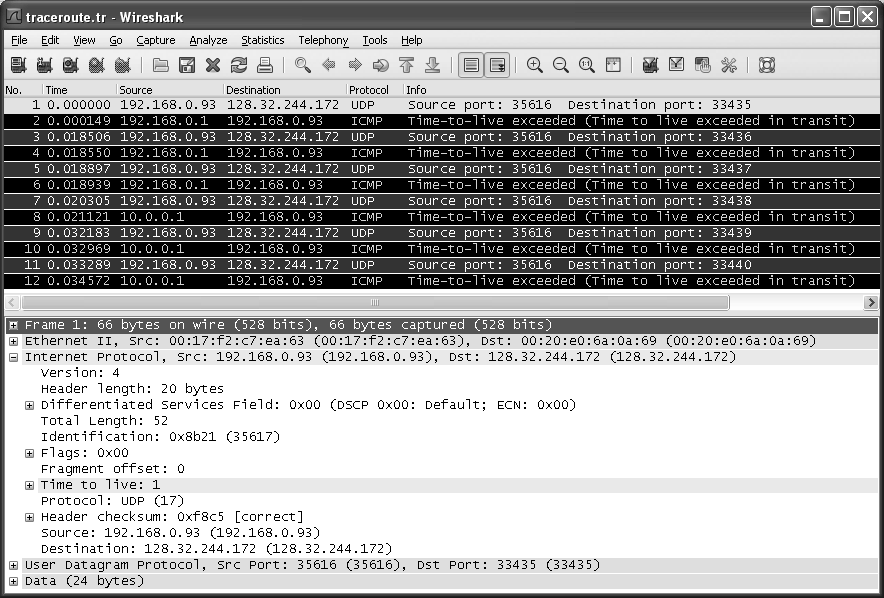
\includegraphics[width=0.7\textwidth]{imgs/8/8-12.png}
	\caption{使用IPv4 的traceroute 以发送一个TTL=1的UDP/IPv4数据报到目的端口号33435开始。在加1和重试之前每个 TTL值将被尝试3次。每个到期数据报导致在恰当跳数距离的路由器发送一个ICMPv4 超时报文返回源头。报文的源地址是“面对”发送者一方的路由器的接口地址}
\end{figure}

在图8-12中,我们能够看到 traceroute发送了6个数据报,每个数据报是按顺序发
送到目的端口号的,以33435开始。如果我们仔细观察会发现,前三个发送的数据报的
TTL = 1,第二组发送的三个数据报的TTL=2。图8-12显示了第一个。每个数据报会导致
发送一个 ICMPv4超时(代码0)报文。前三个是从路由器 N3(IPv4地址192.168.0.1)发出
的,后三个是从路由器N2(IPv4地址 10.0.0.1)发出的。图8-13显示了最后一个ICMP 报
文的详细信息。

这是此追踪的最终ICMP超时报文。它包含了在N2接收时看到的原始的IPv4数据报
(包11)。该数据报到达的时候其TTL=1,但是在递减之后值太小了,以至于 N2 不能执行
额外转发到128.32.244.172的操作。因此,N2向原始数据报的源地址发送一个超时报文。
\begin{figure}[!htb]
	\centering
	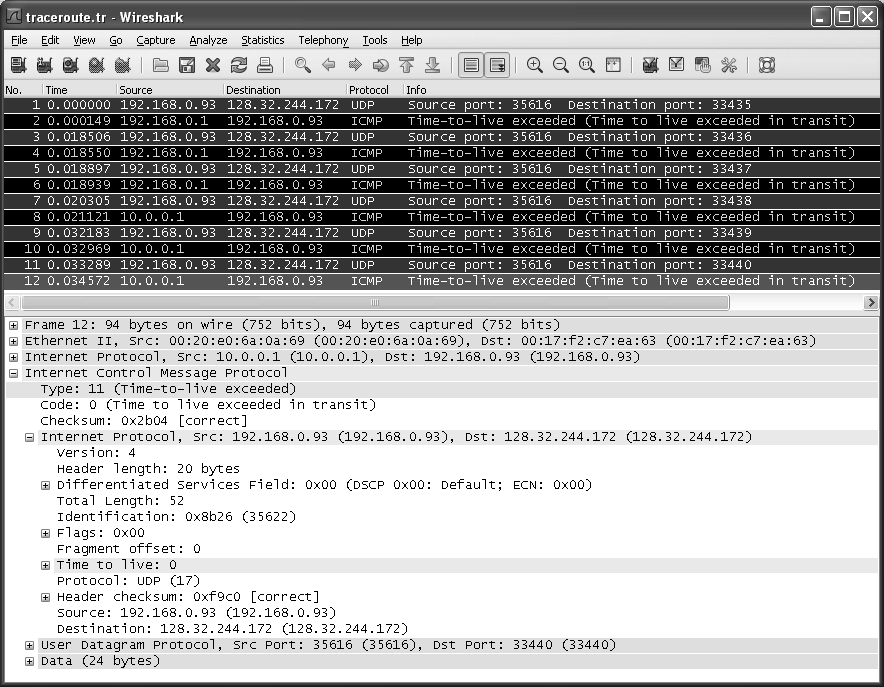
\includegraphics[width=0.7\textwidth]{imgs/8/8-13.png}
	\caption{此追踪中的最后一个 ICMPv4 超时报文是由路由器N2(IPv4地址是10.0.0.1)发出的。它包含了导致产生超时报文的原始数据报的一个拷贝。内部IPv4头部的 TTL字段为0,这是因为N2 将其从1减为0}
\end{figure}

\subsection{参数问题(ICMPv4类型 12,ICMPV6 类型4)}

当一个主机或者路由器接收到一个 IP 数据报,其IP 头部存在不可修复的问题时便会产
生一个ICMP参数问题报文。当一个数据报不能够被处理,且没有其他的ICMP报文来描述
这个问题时,这个报文充当了一个“包罗万象”的错误状态指示器。在ICMPV4 和 ICMPV6
中,当头部中某个字段超过可接受范围导致了一个错误时,一个特殊的ICMP差错报文指
针 (Pointer)字段指示了错误字段相对于出错IP 头部的偏移值。以ICMPv4 为例,指针字
段值为1表示一个错误的IPv4 DS 字段或者ECN字段(这些字段以前称IPv4服务类型
(Type of Service) 或者ToS 字节(ToS Byte),但已经被重新定义和命名过了。参见第5章)。
ICMPv4 的参数问题报文格式如图8-14所示。

代码0是ICMP参数问题报文最为常见的变体,可用于 IPv4头部中出现的任何问题,
尽管当头部或者数据报的总长度字段出现问题时可能会产生代码为2的报文。代码1以前被
用于指示数据包中缺少例如安全标志之类的选项,但目前已经不用了。代码2是最近才定
义的代码,指示存在一个损坏了的IHL 或者总长度字段值(参见第5章)。这个差错报文的
ICMPv6 版本如图8-15所示。

在ICMPv6中,相对于ICMPv4版本,差错的对待方式在某种程度上已经被重新定义
为三种情况:存在错误的头部字段(代码0),存在无法识别的下一个头部(Next Header)类
型(代码1),存在无法识别的IPv6选项(代码2)。与ICMPv4中对应的差错报文一样,
ICMPv6 参数问题中的指针字段给出了相对于问题IPv6 头部的字节偏移。例如,指针字段值
为40 指示第一个IPv6 的扩展头部中存在问题。

图8-14 当没有其他报文可应用时便采用ICMPv4 参数问题报文。指针字段指示了出错的IPv4头部中
出问题的值的字节索引。代码0是为最常见的。代码1以前用于指示缺失了一个必需的选项,
但现在已成为历史了。代码2指示出错的IPv4数据报存在一个错误的IHL 或者总长度(Total
Length)字段

图8-15 ICMPv6 参数问题报文。指针字段给出了相对于发生错误的原始数据报的字节偏移。代码0
表示一个出错的头部字段。代码1表示一个未识别的下一个头部类型,代码2表示出现了一
个未知的IPv6选项

当IPv6 头部中的某个字段包含了一个非法的值时,会导致错误头部(代码0)差错发
生。如果IPv6 下一个头部(头部链)学段包含了一个IPv6实现并不支持的头部类型值的话,
会导致代码为1的差错发生。最终,当收到一个无法识别的IPv6 头部选项时,会导致代码
为2的差错发生。

\section{ICMP 查询/ 信息类报文}

尽管ICMP 定义了一定数量的查询报文,例如地址掩码请求/应答(类型17/18)、时间
戳请求/应答(类型13/14)、信息请求/应答(类型15/16),但是这些功能已经被其他特殊
目的的协议替代(包括 DHCP,参见第6章)。唯一保存下来的广泛使用的ICMP 查询/信息
类报文是回显请求/应答报文,通常称为 ping,以及路由器发现报文。虽然路由器发现机制
在 IPv4 中并未广泛使用,但是与之类似的功能(邻居发现中的一部分)在IPv6 中却是基本
的。此外,ICMPv6 已经被扩展用于支持移动IPv6和具备组播能力的路由器发现。在本节中,
我们将探讨回显请求/ 应答功能,以及用于基本路由器及组播侦听发现(参见第6和9章)
的报文。在接下来的节中,我们将探索 IPv6 中的邻居发现操作。

\subsection{回显请求 / 应答(ping)(ICMPv4 类型 0/8,ICMPv6 类型 129/128)}
一种最为常用的ICMP报文对就是回显请求和回显应答(或者回复)。在ICMPv4 中,
它们的类型分别是8和0,在ICMPv6中它们的类型分别是128 和129。ICMP 的回显请求
报文大小几乎是任意的(受限于最终封装的IP数据报的大小)。收到ICMP 回显请求报文后,
ICMP的实现要求将任何接收到的数据返回给发送者,即使涉及多个IP 分片。ICMP 的回显
请求/ 应答报文格式如图8-16所示。

图8-16 ICMPv4 和ICMPv6 回显请求和回显应答报文格式。请求中的任何可选数据都必须包含在应
答中。NAT使用其中的标识符字段来匹配请求和应答,正如在第7章中讨论的那样
与其他ICMP 查询/信息类报文一样,服务器必须在回复中包含标识符(Identifier) 和序
列号(Sequence Number)字段。

这些报文是通过一个 ping 程序发送的,该程序通常被用于确定 Internet 上的一台主机是
否可达。如果你一度能够“ping”到一台主机,那么几乎确定能够通过其他的方法(远程登
录,其他服务等)访问到它。然而,当和防火墻一起使用时,这就不能完全确定了。

\begin{tcolorbox}
	程序名ping源自于声呐系统中定位物体。ping 程序是 Mike Muuss 编写的,
	他同时也维护了一个有趣的网页来描述它的历史 [PING]。
\end{tcolorbox}

在ping的实现中将ICMP报文的标识符字段设置为某个数,发送主机能够利用它来分
离返回的应答。在基于UNIX的系统中,例如,发送进程的进程ID 通常被放置在标识符字
段。如果有多个 ping 在同一台主机同时运行的话,这样将允许 ping 应用程序识别返回的应
答,因为ICMP 协议不像传输层协议那样有端口号。当涉及防火墙行为时(参见第7章),这
个字段通常被称为查询标识符(Query Identifier)字段。

当一个新的 ping 实例运行时,序列号字段从0开始,并且每发送一个回显请求报文便
增加1。ping 打印出每个返回的数据包的序列号,方便用户查看数据包是否丢失、重排或者
重复了。回忆一下,IP(因此ICMP也是)是一个尽力(best-effort)数据报传递服务,所以
三者中的任何一种情况都有可能发生。但是,ICMP 拥有IP 没有提供的数据校验和。

ping 程序也在传出的回显请求中的可选数据区域中包含了一份本地时间拷贝。这个时间
和数据区域中剩余的内容均包含在返回的回显应答报文中。当应答收到时,ping 程序注意到
了当前时间,用它减去应答中的时间,便得到了一个到达被 ping 的主机的 RTT估计值。由
于只用到了原始发送者的当前时间,因此这个特征不会涉及发送者和接收者之间的时钟同
步。工具 traceroute 中RTT的测量也采用了类似的方法。

先前版本的 ping 程序每秒发送一个回显请求报文,并打印出每个返回的应答。但是,
新的实现增加了输出格式和行为的变化。在Windows 中,默认是发送4个回显请求,每秒
一个,输出一些统计信息,然后退出。-t选项允许 Windows 中的ping程序不断地发送回显
请求直到被用户停止为止。在Linux中,其行就按传统那样—默认是不停运行直到被用
户中断为止。这些年有许多别的ping 变体被开发出来,且有许多别的标准选项。使用某些版
本的ping,可以构建一个包含特殊数据模式的大数据包。这已经被用于在网络通信设备中寻
找依赖于数据的错误。

在下面的例子中,我们发送一个ICMPv4 回显请求到子网广播地址。这个特定版本的
ping 程序(Linux)需要我们使用-b标志指示使用广播地址确实是我们的真实意图(如果没
有该标志将会给出一个警告,因这将会产生大量的网络流量):

\begin{verbatim}
  Linux% ping -b 10.0.0.127
  WARNING:pinging broadcast address
  PING 10.0.0.127(10.0.0.127) from 10.0.0.1:56(84)bytes of data.
  64 bytes from 10.0.0.1:icmp\_seg=0 tt1=255 time=1.290 msec
  64 bytes from 10.0.0.6:icmp\_seq=0 tt1=64 time=1.853 msec(DUP!)
  64 bytes from 10.0.0.47:icmp\_seq=0 tt1=64 time=2.311 msec (DUR!)
  64 bytes from 10.0.0.1: icmp\_seq=1 tt1=255 time=382 usec
  64 bytes from 10.0.0.6:icmp\_seg=1 tt1=64 time=1.587 msec (DUP!)
  64 bytes from 10.0.0.47:icmp\_seg=1 tt1=64 time=2.406 msec (DUP!)
  64 bytes from 10.0.0.1:icmp\_seg=2 tt1=255 time=380 usec
  64 bytes from 10.0.0.6: icmp\_seq=2 tt1=64 time=1.573 msec(DUP!)
  64 bytes from 10.0.0.47:icmp\_seg=2 tt1=64 time=2.394 msec (DUP!)
  64 bytes from 10.0.0.1:icmp\_seq=3 tt1=255 time=389 usec
  64 bytes from 10.0.0.6: icmp\_seq=3 tt1=64 time=1.583 msec(DUP!)
  64 bytes from 10.0.0.47:icmp\_seg=3 tt1=64 time=2.403 msec(DUP!)
  --- 10.0.0.127 ping statistics ---
  4 packets transmitted,4 Packets received,
  +8 duplicates, 08 packet loss
  round-trip min/avg/max/mdev = 0.380/1.545/2.406/0.765 ms
\end{verbatim}

此处,4个传出的回显请求报文被发送出去,我们看到了12个应答。这个行对于采用
广播地址是非常典型的:所有接收节点必须回应。因此,我们看到序列号0、1、2和3,但
是其中每个有3个应答。这个(DUP!)符号表示回显应答中包含的序列号字段和之前接收
到的一样。由于 TTL 值是不同的(255和64),这表明不同类型的计算机正在响应。

注意这个过程(向IPv4的广播地址发送回显请求)能用于快速广播本主机系统的 ARP
表(参见第4章)。这些系统响应回显请求报文,构建一个目的是请求发送者的回显应答报
文。当响应的目标系统位于同一个子网内时,将会触发 ARP 请求查找请求发送者的链路层
地址。这么做,ARP将会在每个响应者和请求发送者之间交换。这也导致回显请求报文的
发送者学习所有响应者的链路层地址。在这个例子中,即使本系统没有关于地址10.0.0.1、
10.0.0.6、10.0.0.47的链路层地址映射,在广播之后便都会出现在ARP 表中。向发送到广播
地址的请求回复ICMP应答报文是可选的。默认情况下,Linux 系统会响应,而Windows XP
系统则不会。

\subsection{路由器发现:路由器请求和通告(ICMPv4类型9,10)}
在第6章,我们看到了 DHCP 是如何被一个主机用于获取IP 地址和学习到附近存在的
路由器的。我们提到的另外一种学习路由器的方式是路由器发现(Router Discovery,RD)。
尽管可以指定为IPv4 和IPv6主机配置,但是由于DHCP 的普及,它在IPv4 中并没有被广
泛使用。但是,目前它被指定与移动IP一起使用,因此我们简要描述一下。这个IPv6版本
构成了 IPv6 SLAAC功能的一部分(参见第6章),在逻辑上是IPv6ND 的一部分。因此,我
们在8.5 节更为广泛的 ND上下文环境中讨论它。

IPv4 的路由器发现是通过采用一对ICMPv4信息类报文实现的\href{https://www.rfc-editor.org/rfc/rfc1256}{[RFC1256]}:路由器请求
(RS,类型10)和路由器通告(RA,类型9)。通告由路由器通过两种方法发送。首先,它
们定期对本地网络(使用TTL =1)的所有主机组播地址(224.0.0.1)进行组播,并提供给
有需要的主机,它们通常使用 RS报文进行请求。使用组播将RS报文发送到所有路由器组
播地址上(224.0.0.2)。路由器发现的主要目的是让一台主机学习到它所在的本地子网中的
所有路由器,因此它能够从中选择一台作为默认路由。它也被用于发现那些愿意充当移动IP
代理的路由器。参见第9章中关于本地网络组播中的详细内容。图8-17给出了 ICMPV4 RA
报文格式,其中包含了一个 IPv4 地址列表可用做主机的默认路由器。

图 8-17 ICMPv4 路由器通告报文包含了一个IPv4地址列表可用作下一跳的默认路由。优先水平允许
网络操作人员为这个列表安排不同的优先级(越高优先级越大)。移动 IPV4\href{https://www.rfc-editor.org/rfc/rfc5944}{[RFC5944]}通过扩
展增强了 RA 报文,目的是为了通告MIPv4 移动代理以及被通告的路由器地址的前缀长度

在图8-17中,地址数(Number of Address)学段给出了报文中路由地址块的个数。每个
块包含了一个IPv4 地址及相应的优先水平(preference level)。地址条目大小(Address Entry
Size)字段给出了每个块的32位字数(在这个例子中是2)。生命周期(Lifetime)字段给出
了地址列表被认为是有效的秒数。优先水平是一个32位的有符号二进制补码整数,其值越
大代表优先级越高。默认的优先水平是0,特殊值 0x80000000表示这个地址不应该用作有
效的默认路由。

RA 报文也被移动 IP\href{https://www.rfc-editor.org/rfc/rfc5944}{[RFC5944]}中的节点用于定位一个移动(即本地和/或外地)代理。
图8-17描述了一个路由器通告报文,其中包含了一个移动代理通告扩展。这个扩展遵循传
统的RA 信息并包含一个值为16的类型(Type)字段,以及一个给出了扩展区域(不包括类
型和长度字段)内字节个数的长度(Length)字段。它的值等于(6+4K),假设包含了K个
地址。序列号字段给出了自从初始化之后代理产生的这种扩展的个数。注册字段给出了发送
代理愿意接受 MIPv4注册的最大秒数(OxFFFF 的表示无穷大)。存在具有以下含义的标志
(Flag)位字段:R(为MIP服务所需的注册),B(代理太忙无法接受新注册),H(代理愿意
充当本地代理),F(代理愿意充当外地代理),M(支持最小封装格式\href{https://www.rfc-editor.org/rfc/rfc2004}{[RFC2004]}),G(代理
支持封装数据报的GRE 隧道),r(保留零),T(支持反向隧道\href{https://www.rfc-editor.org/rfc/rfc3024}{[RFC3024]}),U(支持UDP的
隧道\href{https://www.rfc-editor.org/rfc/rfc3519}{[RFC3519]}),X(支持撤销注册\href{https://www.rfc-editor.org/rfc/rfc3543}{[RFC3543]}),1(外地代理支持区域注册 \href{https://www.rfc-editor.org/rfc/rfc4857}{[RFC4857]})。

除了移动代理通告扩展,还有一个扩展已经被设计用于帮助移动节点。前缀长度扩展
可能位于移动代理通告扩展之后,表示在基本路由器通告中每个对应的路由器地址的前缀长
度。其格式如图8-18所示。

图8-18 ICMPv4可选RA 前缀长度扩展给出了报文中基本路由器通告部分中 N个路由器地址中每个
的显著前缀位数。如果移动代理通告扩展存在的话,这个扩展紧随其后

在图8-18中,长度字段被设置等于N,即来源于基本 RA报文中的地址数字段。每
个8位的前缀长度(Prefix Length)字段给出了在本地子网中使用的路由器地址(Router
Address)字段(图8-17)对应的位数。这个扩展能被移动节点用来确定它是否已经从一个网
络移动到另一个了。采用\href{https://www.rfc-editor.org/rfc/rfc5944}{[RFC5944]}中的算法2,一个移动节点也能缓存一个特定链路上可
用的前缀集合。如果网络前缀集合已经改变,就能检测到是移动了。

\subsection{本地代理地址发现请求 / 应答(ICMPV6 类型 144/145)}
\href{https://www.rfc-editor.org/rfc/rfc6275}{[RFC6275]}定义了4种支持 MIPv6 的ICMPv6报文。其中2个ICMPv6报文用于动态本
地代理地址发现,另外2个用于重新编号和移动配置。当一个 MIPv6 节点访问一个新的网络
时,它使用本地代理地址发现请求报文动态地发现一个本地代理(参见图8-19)。

为了本地前缀,报文被发送到MIPv6本地代理的任播地址。IPv6的源地址通常是移动节点从当前正在访问的
网络上获取的地址(参见第5章)。愿意为给定节点及它的本地前缀充当本地代理的节点会发送一个本地代理地址发现
应答报文(参见图 8-20)。

图8-19 MIPv6本地代理主机发现请求报文包含的标识符将在响应中返回。为了移动节点的本地前
缀,它将被发送到本地代理的任播地址

图8-20 MIPv6本地代理地址发现应答报文包含了来源于对应的请求中的标识符,以及愿意为移动节
点转发数据包的本地代理的一个或者多个地址

直接提供给移动节点单播地址的本地代理地址,极有可能是个移交地址。这些报文用于
处理当一个移动节点在网络中转换但其 HA 已经变化了的情况。在重新建立一个合适的HA
之后,移动节点可能会初始化 MIPv6绑定更新(参见第5章)。

\subsection{移动前缀请求 / 通告(ICMPV6 类型 146/147)}
移动前缀请求报文(参见图8-21)是当一个节点的本地地址就要变无效时,用于从一
个HA处请求一个路由前缀更新。移动节点包含一个本地地址选项(IPv6 目的地址选项,参
见第5章),并使用 IPsec 保护请求(参见第18章)。

图 8-21 当一个移动节点离开去请求一个本地代理提供一个移动前缀通告时,
便发送 MIPv6 移动前缀请求报文

请求报文在标识符字段中包含了一个随机值,用来匹配请求与应答。它和路由器请求报
文类似,但是发送给一个移动节点的HA,而不是本地子网。在这个报文的通告形式中(参
见图8-22),封装的IPv6数据报必须包含一个类型为2的路由头部(参见第5章)。标识符
字段的值和请求报文中的标识符值一样。M(Manged Address,托管地址)字段表示主机应
该使用有状态的地址配置,并避免自动配置。O(Other,其他)字段表示一个有状态的配置
方法提供的是信息而不是地址。通告中包含了1个或者多个前缀信息选项。

图 8-22 MIPv6移动前缀通告报文。标识符字段值和请求中对应字段的值一致。M标志指示地址是由
一个有状态配置机制提供的。O标志表示除了地址之外的其他信息是由有状态的机制提供的

移动前缀通告报文是设计用来通知一个移动中的节点其本地前缀已经改变了。这个报文通
常是使用 IPsec保护的(参见第18章),主要是为了帮助移动节点免受假冒前缀通告的欺骗。前
缀信息选项使用了\href{https://www.rfc-editor.org/rfc/rfc4861}{[RFC4861]}描述的格式,包含了移动节点应该用来配置其本地地址的前缀。
\subsection{移动 IPv6 快速切换报文(ICMPV6 类型154)}
MIPv6 的一个变体 MIPv6定义了快速切换 (fast handovers) \href{https://www.rfc-editor.org/rfc/rfc5568}{[RFC5568]}(称 FMIPv6)。
当一个移动节点从一个网络的接人点(AP)移动到另一个时,它指定的方法可以改善IP层的
切换延迟。这是通过在切换发生之前预测路由器和地址信息来完成的。这个协议涉及对所谓
的代理路由器(proxy router)的发现,它的行为类似于普通路由器,但是移动节点在切换到
一个的网络时需要用到。有对应的ICMPv6 代理路由器请求和通告报文(分别称为 RtSoIPr
和 PrRtAdv)。基本的RtSolPr和 PrRtAdv格式如图8-23所示。

图8-23 用于 FMIPv6 报文的通用ICMPv6报文类型。代码(Code)和子类型(Subtupe) 字段给出了
更深人的信息。请求报文使用代码0和子类型2,可能包含发送者的链路层地址和首选的下
一个接人点链路层地址(如果知道的话)作为选项。通告使用代码0~ 5和子类型3。不同的
代码值表示存在不同的选项、通告是否被请求了、前缀和路由信息是否已经改变、DHCP是
否需要处理

一个移动节点可能有关于它将来使用的AP的地址或者标识符的信息(例如,通过“扫
描”802.11 网络)。RtSoIPr报文使用代码0和子类型2,同时必须包含至少一个选项,即新
接人点链路层地址选项。这是用于指出移动节点请求的信息是关于哪个 AP的。RtSolPr报文
可能也包含一个链路层地址选项来识别源,如果知道的话。这些选项使用了IPv6 ND 选项格
式,因此我们在详细探讨 ND 时再讨论它们。

\subsection{组播侦听查询/ 报告 / 完成(ICMPV6 类型 130/131/132)}
组播侦听发现(MLD)\href{https://www.rfc-editor.org/rfc/rfc2710}{[RFC2710]}\href{https://www.rfc-editor.org/rfc/rfc3590}{[RFC3590]}为采用IPv6的链路提供了组播地址管理。
它和IPv4采用的IGMP协议类似,在第9章中有描述。那一章详细地介绍了IGMP操作和
ICMPv6报文的使用。此处我们描述组成 MLD(版本1)报文的格式,包括组播侦听查询、
报告和完成报文。基本格式如图8-24所示。这些报文被发送时其 IPv6跳数限制(Hop Limit)
字段值1,并带有路由器告警逐跳IPv6选项。

MLD 的主要目的是让组播路由器了解与它们相连的每个链路上的主机使用的组播地址。
MLDv2(版本2组播侦听发现,在下一节描述)扩展了此功能,允许主机指定它们希望(或
不希望)接收流量的特定主机。组播路由器发送两种形式的 MLD 查询报文:一般(general)
的查询和特定于组播地址(multicast-address-specific)的查询。一般来说,路由器发送查询
报文,主机采用报告响应,或者是响应查询,或者是在一台主机的组播地址成员发生变化时

图 8-24 ICMPv6 MLD版本1报文都是这种形式。查询(类型130)都是通用或者特定组播地址的。
一般查询要求主机报告它们正在使用哪个组播地址,特定于地址的查询用于确定一个特定
的地址是否(仍然)在使用。最大的响应时间是主机可能延迟发送响应查询报文的最大毫秒
数。对于一般的查询和针对特定报告查询的组播地址,其目的组播地址为0。对于报告(类型
131)和完成报文(类型132),它将分别包含和报告相关的地址或者不再感兴趣的地址

最大响应时间(Maximum Response Time)字段只有在查询时是非零的,它是响应查询
主机发送报告可能推迟的最大毫秒数。由于组播路由器只需要知道,至少有一台主机对发往
特定组播地址的流量感兴趣(因为链路层组播支持允许路由器不必为每个目的复制报文),节
点可以随机故意地拖延它们的报告,甚至完全抑制它们(如果发现另一个邻居已经做出了响
应)。这一字段提供这种延迟时长的一个上限。对于一般的查询和路由器在报告中感兴趣的
地址,组播地址(Multicast Address)字段为0。对于 MLD 报告报文(类型131)和 MLD完
成报文(类型132),它分别包含和报告相关的地址或不再感兴趣的地址。

\subsection{版本2 组播侦听发现(ICMPV6 类型143)}
\href{https://www.rfc-editor.org/rfc/rfc3810}{[RFC3810]}定义了在\href{https://www.rfc-editor.org/rfc/rfc2710}{[RFC2710]}中描述的MLD功能扩展。特别是,它定义了一个组播
侦听的方式来指定只监听一个特定集合的发送者(或者,排除一个特定的集合)。因此,它
对支持源特定组播(SSM;参见第9章和\href{https://www.rfc-editor.org/rfc/rfc4604}{[RFC4604]}\href{https://www.rfc-editor.org/rfc/rfc4607}{[RFC4607]})非常有用。它基本上是对
与IPv4一起使用的IGMPv3协议在IPv6 下使用的一个转换,它使用ICMPv6 来管理多数
组播地址。因此,我们将在这里描述报文格式,但组播地址动态的操作将在第9章中介绍。
MLDv2扩展了MLD 查询报文,增加了与特定来源相关的其他信息(见图8-25)。报文中开
始的24个字节和 MLD格式是一样的。

最大响应代码(Maximum Response Code)字段指定发送 MLD 响应报文之前允许的最大
时间。这个字段的值是特殊的,因此其解释与 MLDvI 也略有不同:如果它小于 32 768,则
与 MLDV1 中一样,最大的响应延迟就设置为该值(以毫秒为单位)。如果该值等于或大于
32769,字段使用图8-26所示的格式编码一个浮点数。

在这种情况下,最大响应时间设置为等于((mant | 0x1000)<<(exp +3))毫秒。采用这个
看似复杂的编码策略的原因是为了让大、小响应延迟值都能编码在这个字段中,并保留一
些与 MLDv1的兼容性。特别是,它可以仔细调整离开延迟,并影响报告的突发性(参见第

8-25 MLDv2 查询报文格式,它与 MLD版本1报文通用格式兼容,最大的区别是能够从主机感兴
趣列表中限制或者剔除特定的组播源

当最大响应代码字段值至少为32768时,MLDv2查询报文使用的浮点格式。在这些情况中
延迟被设置为((mant| 0x1000)<<(exp +3))毫秒

一般查询中组播地址字段设置为0。对于一个特定组播地址查询或特定的组播地址和源
询,它被设置查询的组播地址。S字段指示是否应抑制路由器端处理。设置时,它表示
王何接收的组播路由器,当监听到一个查询时它必须抑制正常的计时器更新计算。这并不表
,如果路由器本身就是一个组播监听者的话,查询器选举或正常的“主机端”处理应该初

如果设置了 QRV (Querier Robustness Variable,查询器鲁棒性变量)字段,它将包含一
个不超过7的值。如果发送者的内部QRV 值超过7,那么这个字段应设为0。在第9章介绍
的鲁棒性变量能够根据一个子网上的丢包率来微调 MLD 的更新率。QQIC (Querier’s Query
Interval Code,查询器查询间隔代码)字段编码查询时间间隔,如图8-27所示。


图8-27 MLDv2 查询器查询间隔代码编码了 MLDv2 查询之间的时间间隔。这个值的(未编码)版
本称为查询器查询间隔,且是以秒来测量的。QQ1是通过下面的方法来计算的:如果
QQIC<128,QQ1 = QQIC;否则 QQ1= ((mant | 0x10)<<(exp +3))

查询时间间隔以秒为单位,它从 QQIC字段按如下方式计算得到:如果QQIC<128,那
么 QQ1=QQIC;否则,QQ1=((mant | 0x10)<<(exp+ 3))。

源个数(Number of Sources)(N) 字段表示查询中源地址个数。对于一般的查询或者特
定的组播地址查询,此字段为0。对于特定的组播地址和源查询报文,它不为0。

MLDv2 报告中使用的组播地址记录(参见图8-28和图8-29)包含对IPv6 节点源地址过
滤器所做的修改(参见第9章关于组播在这种过滤器操作上的更多信息,描述了对特定接收
主机感兴趣或者不感兴趣的发送主机集合)。

图8-28 MLDv2 报告报文包含了一组组播地址记录向量

记录类型主要可以分为三类:当前状态(current state)记录,过滤模式变化(filter mode
change)记录和源列表改变(source list change)记录。第一类包括 MODE IS INCLUDE (IS
IN)和 MODE\_IS\_EXCLUDE (IS\_EX)类型,指明的地址过滤模式对于指定的源而言(其中
必须至少存在一个)分别是“包括”或“排除”。过滤模式变化类型 CHANGE\_TO\_INCLUDE
(TO\_IN)或CHANGE\_TO\_EXCLUDE(TO\_EX)和当前状态记录是类似的,但当有变化或
者不需要包含一个非空的源列表时将被发送。源列表改变类型,当过滤器的状态(包含/排
除)不变而只有源列表被改变时,ALLOW\_NEW\_SOURCES(ALLOW)和BLOCK\_OLD
SOURCES(BLOCK)将被使用。为了简化了MLDV2\href{https://www.rfc-editor.org/rfc/rfc5790}{[RFC5790]} 的操作,对MLDv2(和
IGMPv3)做了修改,即删除了 EXCLUDE 模式。这种“轻量级”的方法,称为LW-MLDV2
(和LW-IGMPv3),使用先前定义的相同报文格式,但删除了很少使用的要求组播路由器保存
附加状态的 EXCLUDE指令。

图8-29 一条组播地址(组)记录。MLDv2报告报文中可能存在多个这样的记录。记录类型字段
值是下列之一:MODE\_IS\_INCLUDE,MODE\_IS\_EXCLUDE, CHANGE\_TO\_INCLUDE \_MODE,
CHANGE\_TO\_EXCLUDE\_MODE, ALLOW\_NEW\_SOURCES,或BLOCK\_OLD\_SOURCES。
LW-MLDv2 通过删除 EXCLUDE 模式简化了 MLDV2。辅助数据长度(Aux Data Len) 字段包
含了记录中的辅助数据,以32位字为单位。对于在\href{https://www.rfc-editor.org/rfc/rfc3810}{[RFC3810]}中定义的MLDv2 而言,此字
段必须为 0.表示没有辅助数据

\subsection{组播路由器发现(IGMP 类型 48/49/50,ICMPV6 类型 151/152/153)}
\href{https://www.rfc-editor.org/rfc/rfc4286}{[RFC4286]} 描述组播路由器发现(Multicast Router Discovery,MRD),该方法定义的特
殊报文可以和ICMPv6 和IGMP一起使用,用来发现能够转发组播数据包和它们的一些配置
参数的路由器。最初的想法主要是和“IGMP/MLD侦听”一起使用。IGMP/MLD 侦听是一
种机制,主机和路由器(例如,第2层交换机)以外的系统也可以了解网络层组播路由器和
感兴趣主机的位置。我们将在第9章IGMP上下文中详细地讨论它。MRD报文发送时总是
将IPv4的TTL 或IPv6 的跳数限制字段设1,并设有路由器警告选项,可能是如下类型之
一:通告(151),请求(152),或终止(153)。在配置的时间间隔定期地发送通告,表明路
由器愿意转发组播流量。终止报文表明要终止这种意愿。请求报文可用于请求路由器发送通
告报文。通告报文格式如图8-30所示。

图 8-30 MRD的通告报文(ICMPv6 类型151;IGMP 类型48)包含说明多长时间发送主动通告的通
告时间间隔(秒)、发送者的查询间隔(QQI)和 MLD定义的鲁棒性变量。发送者的IP地址
就是用来指示接收者能够转发组播流量的路由器。该报文被发送到所有侦听者的组播地址
(IPV4,224.0.0.106; IPv6, ffO2::6a)

通告报文从路由器的IP地址(IPv6链路本地地址)发送到所有侦听者的IP 地址:
224.0.0.106(IPv4)和链路本地组播地址 ff02::6a(IPv6)。接收者能够了解路由器的通告间
隔和 MLD 参数(QQ1和QRV,在第9章中详细介绍)。请注意,QQ1 值是查询的间隔(以秘
计),不是之前在 MLDv2 查询中描述的QQIC(编码版本的QQ1值)。

请求和终止报文格式几乎相同(见图8-31),只有类型字段的值有所不同。

图 8-31
ICMPv6 MRD 请求(ICMPv6 类型 152;IGMP 类型 49)和终止(ICMPv6 类型153;IGMP类
型50)报文使用相同的格式。MRD报文将IPv6跳数限制字段或者IPv4 TTL 字段值设置为1,
并包含路由器警告选项。请求被发送到所有路由器的组播地址(IPv4,224.0.0.2;IPv6, ff02::2)

图8-31显示请求和终止报文的格式几乎是相同的。请求报文请求一个组播路由器发送
一个通告报文。这样的报文被发送到所有路由器地址224.0.0.2(IPv4)和本地链路组播地址
f02::2(IPv6)。终止报文被发送到所有的侦听者IP 地址,表示发送路由器不再愿意转发组
播流量了。

\section{IPV6 中的邻居发现}

IPv6中的邻居发现协议(有时简称为 NDP 或者 ND)「RFC48611将路由器发现和田
ARP提供的带有地址映射功能的ICMPv4重定向机制结合在一起。它也被指定用于支持移动
IPv6。与ARP和IPv4 普遍使用广播地址(除了路由器发现)不同,ICMPv6广泛使用组播地
址,在网络层和链路层中都使用。(回忆第2 章和第5章,IPv6 甚至没有广播地址。)

ND 被设计允许在同一个链路或者网段的节点(路由器和主机)找到彼此,确定它们之
间是否有双向连通性,确定一个邻居是否变得不合作或者不可用。它也支持无状态的地址自
动配置(参见第6章)。所有的ND功能都是由网络层或者之上的ICMPv6提供的,致使它最
大限度地独立于底层所采用的链路层技术。但是,ND 并不倾向于采用链路层组播功能(参
见第9章),也正是这个原因在非广播和非组播链路层(称为非广播多路访问或者 NBMA链
路)上的操作可能会有一些差别。

ND 中两个主要部分是:邻居请求/通告(NS/NA),在网络和链路层地址之间提供类似
于ARP的映射功能;还有路由器请求和通告(RS/RA),提供的功能包括路由器发现、移动
IP 代理发现、重定向,以及对一些自动配置的支持。ND 的一个安全变体 SEND\href{https://www.rfc-editor.org/rfc/rfc3971}{[RFC3971]}
通过引人额外的ND选项增加了认证和特殊形式的寻址。

ND报文就是ICMPv6报文,只是发送时IPv6的跳数限制字段值被设置为255。接
收者通过验证进来的ND报文有这个值,以防止被非本链路上的发送者尝试发送假冒本地
ICMPv6报文(这样的报文到达时其值会小于255)欺骗。ND报文可以携带丰富的选项。首
先我们讨论主要的报文类型,然后详述可用的选项。

\subsection{ICMPv6 路由器请求和通告(ICMPV6 类型 133,134)}
路由器通告(RA)报文表明附近路由器的存在及其功能。它们定期被路由器发送,或者
是响应一个路由器请求(RS)报文。RS报文(参见图8-32)用于请求链路上的路由器发送
RA 报文。RS报文被发送到所有路由器组播地址 ff02::2。如果报文的发送者使用IPv6地址,
而不是未指定的地址(在自动配置过程中使用),则应该包括一个源链路层地址选
项。对于这样的报文,这是唯一有效的选项 \href{https://www.rfc-editor.org/rfc/rfc4861}{[RFC4861]}。

路由器通告(RA)报文(参见图8-33)是由路由器发送到所有节点的组播地址
(FF02:1)的,或者是发送到请求主机的单播地址——如果该通告是为了响应一个
请求。RA报文通知本地主机和其他路由器关于本地链路的有关配置细节。

ICMPv6 路由器请求报文非常简单,但是通
常包含一个源链路层地址选项(不像ICMPv4
中的对应项)。假如链路中使用了一个不常用
的MTU 值,那么它可能包含一个 MTU选项

当前跳数限制(Current Hop Limit)
字段指定主机发送IPv6数据报的默认跳数限制。值为0表示发送路由器并不关心。下一个
字节包含了位字段数,正如在\href{https://www.rfc-editor.org/rfc/rfc5175}{[RFC5175]} 总结和扩展的那样。M(托管)字段表明本地 IPv6
地址分配是由有状态的配置来处理的,主机应避免使用无状态的自动配置。0(其他)字段
表示其他有状态的信息(即 IPv6地址以外的)使用一个有状态的配置机制(见第6章)。H(本
地代理)字段表示发送路由器愿意充当一个移动IPv6 节点的本地代理。Pref(优先级)字段
给出了将报文发送者作为一个默认路由器来使用的优先级层次:01,高;00,中(默认);
11,低;10,保留(未使用)。有关这一字段的更多细节在「RFC41911中有描述。当和实验
性质的ND代理工具\href{https://www.rfc-editor.org/rfc/rfc4389}{[RFC4389]}配合使用时,将使用P(代理)标志。它为IPv6 提供了一个
类似代理 ARP的功能(见第4章)。

一个ICMPv6路由器通告报文被发送到所有节点的组播地址(02 :1)。接收节点检查以确
定跳数限制字段值是255,并确保数据包尚未通过路由器转发。报文包括三个标志:M(托管
地址配置),O(其他有状态的配置)和H(本地代理)

路由器生命周期(Router Lifetime)字段表示发送路由器可以作为默认下一跳的时间,
以秒计。如果它被设置为0,发送路由器不应该用作默认路由器。此字段只适用于使用发
送路由器作为默认路由器,它不会影响同一个报文中的其他选项。可达时间(Reachable
Time)字段给出一个节点到达另一个节点所需的毫秒数,假设已经发生了双向通信。这被
邻居不可达检测(Neighbor Unreachability Detection) 机制使用(见8.5.4节)。重传计时器
(Retransmission Timer)字段规定主机延迟发送连续ND报文的时间,以毫秒为单位。

此报文通常包含源链路层选项(如果适用的话),如果链路中使用了可变长度的MTU则
应包含MTU选项。该路由器还应该包括前缀信息选项,表示本地链路上使用了哪些IPv6前
缀。第6章包含了一个如何使用RS和RA 报文(例如,参见图6-24和图6-25)的例子。

\subsection{ICMPV6邻居请求和通告(ICMPV6 类型 135,136)}
ICMPv6 中的邻居请求(NS)报文(参见图8-34),有效地取代了IPv4 中的ARP请求报
文。其主要目的是将IPv6地址转换为链路层地址。但是,它也被用于检测附近的节点是否
可达,它们是否可以双向到达(即节点间是否可以互相通信)。当用于确定地址映射时,它
被发送到目标地址(Target Address)字段中包含的IPv6地址所对应的请求节点的组播地址
(前缀f02::1:/104,并结合请求IPv6地址中的低24位)。关于如何使用请求节点组播寻址的
更多细节,请参阅第9章。当这个报文被用来确定到邻居的连接性时,它被发送到该邻居的
IPv6 单播地址,而不是请求节点的地址。

NS报文包含发送者想设法学习的链路层地址对应的IPv6地址。该报文可能包含源链路
层地址选项。当请求是被发送到一个组播地址时,该选项必须包含在使用链路层寻址的网络
中,对于单播请求而言,该选项应该被包含。如果报文的发送者使用未指定的地址作为源地
址(例如,在重复地址检测期间),则不应该包括该选项。

ICMPv6 邻居通告(NA)报文(参见图8-35)和IPv4 中的ARP 响应报文的目的一样,
还能够有助于邻居不可达检测(见8.5.4节)。它要么作NS报文的响应被发送,要么当一
个节点的IPv6地址变化时被异步发送。它要么被发送到请求节点的单播地址,要么当请》
节点使用未指定的地址作为源地址时,它被发送到所有节点的组播地址。

图8-34 ICMPv6 邻居请求报文和 RS报文类似,但包含一个目标IPv6地址。这些报文被发送到请求
节点组播地址以提供类似于 ARP的功能,发送到单播地址以测试到其他节点的可达性。在使
用低层寻址的链路上,NS报文包含源链路层地址选项


图 8-35
ICMPv6邻居通告报文包含以下标志:R表示发送者是一个路由器,S表示通告是为了响应一
个请求,O表示该报文的内容应覆盖其他缓存的地址映射。目标地址字段包含报文发送者的
IPv6地址(一般,从ND 请求中请求节点的单播地址)。包含一个目标链路层地址选项用于为
IPv6启用类似的ARP 功能

R(路由器)字段表示该报文的发送者是一个路由器。这可能会改变,例如当一台路由
器不再是路由器,而成为一台主机时。S(请求)字段表示该报文是在响应先前收到的请求。
这个字段用来验证已经取得的邻居之间的双向连通性。0(覆盖)字段表示在报文中的信息
应覆盖报文发送者之前缓存的任何信息。它不应该在请求通告、任播地址或请求代理通告中
设置,而应该在其他通告(请求或主动)中设置。

对于请求通告,目标地址字段就是正在被查找的IPv6地址。对于主动通告,它是已经
改变的链路层地址对应的IPv6地址。当通告是通过一个组播地址被请求时,此报文必须包
含支持链路层寻址的网络的目标链路层地址。我们现在来看一个简单的例子。

\subsubsection{例子}

在这里我们看到ICMPv6 回显请求/应答与ND一起使用的结果。发送者是一台启用了
IPv6 的Windows XP 系统,在附近的Linux 系统上捕获数据包。为清晰起见,有些行已被隐藏。
\begin{verbatim}
    
C:\> ping6 -s fe80::210:18ff:fe00:100b fe8o::211:11ff:fe6f:c603

Pinging fe8O::211:1lff:fe6f:c603

from fe80::210:18ff:fe00:100b with 32 bytes of data:

Reply from fe80::211:11ff:fe6f:c603: bytes=32 time<1ms

Reply from

fe80::211:11ff:fe6f:c603: bytes=32 time<1ms

Reply from fe8O::211:11ff:fe6f:c603:bytes=32 time<1ms

Reply from fe80::211:11ff:fe6f:c603:bytes=32 time<1ms

Ping statistics for fe80::211:11ff:fe6f:c603:

Packets: Sent = 4, Received = 4,Lost = 0 (08 10ss),

Approximate round trip times in milli-seconds:

Minimum = Oms,Maximum = 0ms,Average =0ms

Linux# tcpdump -i etho -$1500 -w -P ip6

tcpdump:1istening on ethO,

1ink-type EN1 OMB (Ethernet),capture size 1500 bytes

1 21:22:01.389656 fe80::211:11ff:fe6f:c603 > Ef02::1:ff00:100b:

[icmp6 sum ok]icmp6:neighbor sol: who has

fe80::210:18ff:fe0o:100b

(srC 1laddr: 00:11:11:6f:c6:03)

(len 32,hlim 255)

2 21:22:01.389845 fe80::210:18ff:fe00:100b > fe80::211:11ff:fe6f:c603:

[icmp6 sum ok] icmp6: neighbor adv:tgt is

fe80::210:18ff:fe00:100b(SO)

(tgt 1laddr: 00:10:18:00:10:0b)

(len 32,hlim 255)

3 21:22:02.390713 fe80::210:18ff:fe00:100b > fe80::211:11ff:fe6f:c603:

[icmp6 sum ok]icmp6: echo request seg 18

(len 40,hlim 128)

4 21:22:02.390780 fe80::211:11ff:fe6f:c603 > fe80::210:18ff:fe00:100b:

[icmp6 sum ok]icmp6:echo reply seg 18

(len 40,hlim 64)

continues
\end{verbatim}

Windows XP 和 Linux 均提供了 ping6程序(最近版本的 Windows 将 IPv6功能纳人常规
的ping 程序)。-s选项告诉它使用的源地址。回想一下在IPv6 中一个主机可能有可供选择
的多个地址,在这里我们选择了一个链路本地地址 fe80::211:11ff:fe6f:c603。跟踪显示了 NS/
NA 交换和一个ICMP 回应请求/应答对。通过观察可知所有 ND 报文的IPv6跳数限制字段
值为255,ICMPv6 回显请求和回显应答报文使用的值为128或64。

NS报文被发送到组播地址 f02:1:f800:100b,就是被请求的IPv6 地址 (fe80:210:18ff:fe00:
100b)对应的请求节点的组播地址。我们看到请求节点在源链路层地址选项中还包括它自己
的链路层地址 00:11:11:6f:c6:03。

NA应答报文使用链路层(和IP 层)单播地址被发送回请求节点。目标地址字段包含请
求报文中请求的值:fe80::210:18ff:fe00:100b。此外,我们还看到S和O标志字段被设置,
表示该通告为了响应先前的请求,所提供的信息应该覆盖其他任何请求节点可能缓存的信
息。R 标志字段并未设置,表示响应的主机并不充当路由器。最后,请求节点包括在目标链
路层地址选项中最重要的信息:请求节点的链路层地址 00:10:18:00:10:0b。

\subsection{ICMPV6 反向邻居发现请求/通告(ICMPV6 类型141/142)}

IPv6\href{https://www.rfc-editor.org/rfc/rfc3122}{[RFC3122]} 中的反向邻居发现(Inverse Neighbor Discovery,IND) 功能起源于需要
在帧中继网络中确定给定的链路层地址对应的IPv6地址。它类似于反向的ARP 协议,主要
用于支持IPv4网络中的无盘计算机。其主要功能是确定一个已知的链路层地址对应的网络
层地址。图8-36显示了 IND 请求和通告报文的基本格式。

IND 请求报文被发送到IPv6层的所有节点的组播地址,但是却封装在
一个单播链路层地址(正在被查找的那个)中。它必须同时包含源链路层地址
选项和目的链路层地址选项。它可能也包含一个源/目标地址列表选项和/
或一个MTU选项。

图8-36 ICMPv6 IND 请求(类型 141)和通告(类型142)
报文的基本格式相同。它们被用于从已知的链路层地址映射到 IPV6地址

\subsection{邻居不可达检测}

ND 的一个重要特征是检测在同一个链路上的两个系统什么时候丢失了或者变得非
对称了(即在两个方向上均不可用)。这是通过邻居不可达检测(Neighbor Unreachability
Detection,NUD)算法完成的。它被用于管理每个节点上的邻居缓存(neighbor cache)。邻
居缓存和第4章中描述的 ARP缓存类似,它是一个(概念上)数据结构,用于保存IPv6到
链路层地址的映射信息(这些信息在执行到链路邻居的IPv6数据报直接交付时需要),以及
针对映射状态的信息。图8-37显示了它如何在邻居缓存中维护条目。

图8-37 邻居不可达检测帮助维护由多个邻居条目组成的邻居缓存。在任何时间,每个条目是5种状
态中的一种。对连接可达性的确认是通过接收邻居通告报文或者其他更高层的协议信息来完
成的。主动证据包括主动的邻居和路由器通告报文

每个映射可能是如下5个状态中的一种:INCOMPLETE, REACHABLE, STALE, DELAY,
PROBE。图8-37所示的转换图显示的初始状态是 INCOMPLETE 或 STALE。当一个 IPv6 节点
有一个单播数据报需要发送到目的地时,它会检查其目标缓存(destination cache),看一看对应
于目的地的条目是否存在。如果存在且目的地是在链路上的,再查看邻居缓存,确定邻居状态
是否是 REACHABLE。如果是,使用直接交付方式发送数据报(见第5章)。如果没有邻居缓存
条目,但目标似乎是在链路上,NUD 会进入 INCOMPLETE状态,并发送一个NS报文。成功
收到一个请求 NA报文便可以确定该节点是可达的,条目进入 REACHABLE 状态。STALE 状态
对应于目前还未确认的无效条目。当一个条目之前是 REACHABLE 状态但已有一段时间没有
更新,或者收到主动报文时(例如,一个节点改变其地址并发送主动 NA报文),它就进人这
个状态。这些情况表明,有可能是可达的,但仍需要一个有效的NA 来确认。

其他状态 DELAY 和 PROBE 是临时状态。DELAY 被用于当一个数据包已经被发送了,
但ND目前尚无证据表明可能是可达的情况。该状态给上层协议一个机会来提供更多的证
据。如果在 DBLAY \_FIRST\_PROBE\_TIME 秒(常数)后仍然没有接收到证据,状态将会改
变到 PROBE。在PROBE状态,ND 会定期发送NS报文(每 RetransTimer 毫秒,常数默认
值 RETRANS\_TIMER 等于1000)。如果在发送 MAX\_UNICAST\_SOLICIT(预设为3)个
NS报文后还未收到任何证据,就应该删除该条目。

\subsection{安全邻居发现}
SEND(安全邻居发现)\href{https://www.rfc-editor.org/rfc/rfc3971}{[RFC3971]}是一组特殊的增强功能,旨在为ND报文提供额外的
安全性。这是为了帮助抵制各种欺骗攻击,其中一台主机或路由器可能会伪装成另一个(更
多细节见第18章、8.6节和 \href{https://www.rfc-editor.org/rfc/rfc3756}{[RFC3756]})。特别是在响应NS报文时,它防止节点伪装成其他
节点。SEND 不使用IPsec(见第18章),它有自身的特殊机制。这种机制也可用于确保安全
的 FMIPv6 切换 \href{https://www.rfc-editor.org/rfc/rfc5269}{[RFC5269]}。

SEND在一套假设的框架中操作。首先,每个具备SEND的路由器有一个证书
(certificate) 或密码认证,它可以用来证明一台主机的身份。接下来,每个主机还配备了一个
信任锚(trust anchor)—一配置信息可以用来验证证书的有效性。最后,每个节点在配置它
将使用的IPv6地址时,将会生成一个公钥/私钥对。第18章将对证书、信任锚、密钥对以
及其他相关的安全技术进行详细介绍。

\subsubsection{密码生成地址}
也许 SEND 最有趣的特征是使用完全不同类型的称密码生成的地址(Cryptographically
Generated Address, CGA)\href{https://www.rfc-editor.org/rfc/rfc3972}{[RFC3972]}\href{https://www.rfc-editor.org/rfc/rfc4581}{[RFC4581]}\href{https://www.rfc-editor.org/rfc/rfc4982}{[RFC4982]} 的IPv6地址。这种类型的地址是
基于节点的公钥信息,从而将地址和节点证书关联起来。因此,拥有相应的私钥的节点或地
址的所有者能够证明它是一个特定CGA 的授权用户。CGA 也编码与它们相关联的子网前缀,
因此它们不能被轻易地从一个子网转移到另一个子网。这种做法与通常分配地址的方法完全
不同。

将一个64位的子网前缀和一个特殊构造的接口标识符相“或”,便生成了一个IPv6
CGA。CGA 接口标识符是通过一个称为Hashl 的安全散列函数(secure hash function)计
算出来的(被认为难以反转的散列函数,参见第18章),它的输入是节点的公钥和一个特殊
的CGA 参数数据结构。这些参数也被用来作为另一个安全散列函数 Hash2 的输人,它提供
了散列扩展(hash extension)技术,能有效地扩展散列函数的输出位数,进而提高其安全
性(即生成一个不同的输人但却有相同散列值的强度)[A03]\href{https://www.rfc-editor.org/rfc/rfc6273}{[RFC6273]}。CGA 技术允许自动
生成地址所有者的公钥,所以这种方法可以在没有公钥基础设施(public key infrastructure,
PKI) 或其他可信任的第三方下工作。

CGA 参数数据结构如图8-38所示。伪随机序列(Modifier)字段初始化一个随机值,碰
撞计数(Collision Count)字段初始化次0。这个结构包括一个扩展字段(Extension Field)可
供未来使用\href{https://www.rfc-editor.org/rfc/rfc4581}{[RFC4581]}。

 Hashl:最上面的64位安全散列函数的所有字段值,包括在计算 Hash2时
发现的最终伪随机序列值。

Hash2:最上面的112位的安全散列函数字段值,其中子网前缀和碰撞计数
零。通过增加伪随机序列字段来重新计算 Hash2,直到最初(16*Sec)位变
0为止。

图8-38 用来计算CGA的SEND方法。CGA 参数数据结构可用作两个加密散列函数 Hashl 和 Hash2
的输入。Hash2值必须有(16*Sec)个初始0位,其中 Sec 是一个3位的参数。到Hash2适
当计算时,才改变伪随机序列字段。结果值被用来计算 Hashl,并和Sec与子网前缀结合用
来生成 CGA

一个称为 Sec 的3位无符号参数将影响该方法对数学破解的抵御力(采用了安全散列函
数\href{https://www.rfc-editor.org/rfc/rfc4982}{[RFC4982]}),以及计算中的计算复杂性(在 Sec 值中它们是指数的)。IANA 为 Sec 值维护
一个注册表[SI]。配合 Sec值,Hashl 和 Hash2 函数在相同的CGA参数块进行操作。该地
址所有者首先为伪随机序列字段选择一个随机值,将子网前缀字段看作0,再计算Hash2的
值。结果需要有(16*Sec)个初始0位,所以修改输人将伪随机序列字段递增1,并重新计
算 Hash2 直到条件满足为止。这种计算的时间复杂度为 O(216S0o),并随着Sec 的增加代价会
更高。但是,只有当最初创建地址时,这种计算才是必需的。

一旦找到适当伪随机序列字段,便用59位的Hashl值形成接口标识符的低59位。前
3位构成3位Sec 值,6~7(左起)位包含两个0位(对应于第2章中描述的u和g地址)。
如果该地址被发现存在冲突(例如,使用第6章描述的重复地址检测),递增碰撞计数字段,
并重新计算 Hash1。碰撞计数值的增长是不允许超过2的。由于地址冲突在开始时是不常见
的,当多个这样的冲突出现时应考虑是否配置错误或遭到了攻击。一旦所有必要的计算完成
了,通过连接子网前缀,Sec 值以及 Hashl值便能形成CGA。需要注意的是,如果子网前
缀改变了,只需要重新计算 Hash1,因为伪随机序列字段值仍然保持不变。(对替代 CGA 的
方法感兴趣的读者应该看看\href{https://www.rfc-editor.org/rfc/rfc5535}{[RFC5535]},它描述了基于散列的地址(hash-based address),或
HBA。HBA 用在一个稍微不同的环境中的多前缀多宿主主机中,并使用了计算复杂度较低
的不同加密形式,当然也定义了 HBA-CGA 兼容选项。)

到目前为止我们已经看到CGA 是如何产生的,但还不知道如何用于安全中。注意任
何人都可以生成一个 CGA,只要有子网前缀、Sec 值和自己的(或别人的)公钥。为了确
保CGA 格式完好,并使用了适当的子网前缀,它必须经过验证,这一过程称为CGA验证
(CGA verification)。一个验证需要CGA 和CGA 参数的知识。验证过程需要确保满足如下条
件:碰撞计数不大于2,CGA 子网前缀和CGA 参数中的前缀匹配,从CGA 参数计算出的
Hashl需要和CGA 的接口标识符部分匹配(其中开始的3位、第6位和第7位“不需要关
心”),通过值为0的子网前缀(Subnet Prefx)和碰撞计数(Collision Count)字段以及 CGA
参数计算出来的 Hash2值应该有(16*Sec)个初始的0位。如果这些检查都是成功的,就是
一个对应于子网前缀的合法CGA。这个计算最多涉及两个散列函数,这是远远比地址生成
过程简单的。

验证CGA 正在被其授权地址所有者使用,这称为签名验证(signature verification),所
有者形成了一个类型报文,并附上一个 CGA 签名,该签名是使用CGA 中的公钥及其对应的
私钥的知识计算出来的。通过将一个特的128位类型标签和报文结合起来,验证将形成一
个数据块。使用一个 RSA 签名(RSASSA-PKCSI-VL\_5 \href{https://www.rfc-editor.org/rfc/rfc3447}{[RFC3447]}),并结合公钥(从 CGA
参数提取)、数据块和签名作为参数来验证CGA的所有权。一般来说,只有在CGA 验证和
签名验证过程都顺利完成时,CGA 及其用户才被认为是合法的。

使用ICMPv6报文和6个在\href{https://www.rfc-editor.org/rfc/rfc3971}{[RFC3971]}中定义的选项来处理CGA 和验证。RFC还定义
了2个IANA托管的注册表,用来保存信任锚选项中的名称类型(Name Type)字段和证书
选项中的证书类型(Cert Type)字段(见8.5.6.13节)。\href{https://www.rfc-editor.org/rfc/rfc3972}{[RFC3972]}定义了CGA报文类型注
册表,采用在\href{https://www.rfc-editor.org/rfc/rfc3971}{[RFC3971]}中定义的128位值(其他值是在SEND之外定义使用的)0x086FC
ASE10B200C99C8CE00164277C08。Sec 的注册值在\href{https://www.rfc-editor.org/rfc/rfc4982}{[RFC4982]}中定义,但目前只提供值0、1、
2,分别对应于在Hash2函数中使用的SHA-1 安全散列函数使用的0、16或32个初始0位。
在\href{https://www.rfc-editor.org/rfc/rfc4581}{[RFC4581]}中定义的扩展格式支持TLV 编码,可用于未来标准的扩展,但到目前为止只
定义了一个[RFCS535]。我们现在将描述两个与SEND一起使用的ICMPv6 报文,等我们在
下一节讲完所有的ICMPv6选项才讨论这些选项。

\subsubsection{证书路径请求/通告(ICMPv6 类型148/149)}
SEND定义了请求和通告报文用来帮助主机确定构成一个证书路径的证书。这被主机用
来验证路由器通告的真实性。图8-39显示了请求报文。

证书路径请求报文包含一个随机标识符(Identifer)学段用来匹配请求和通告。
组件字段值提供了一个索引以表示请求者感兴趣的证书路径中的点。如果需要整个
路径中的证书,这个值被设置全1(值65535)。这个报文可能包含一个信任锚选
项(参见8.5.6.12节)。第18章详细描述了证书和证书路径。

图8-39 证书路径请求报文。发送者通过由组件(Component)字段值提供的位置索引来请
求一个特定的证书。值65535表示需要路径中的所有证书,其中该路径的根身份在
附加信任锚选项中给定

图8-40显示的证书路径通告报文提供了在一个多组件通告中表示一个组件(证书)的方
法。这些报文为了响应一个请求而发送,或由具备SEND功能的路由器定期发送。当为了响
应请求而发送报文时,目的IPv6地址是接收者的被请求节点组播地址。

请求路径通告报文。发送者通过由组件字段值提供的位置索引来请求一个特定的证书。值
65535 表示需要所有根植在一个附加信任锚选项中给定身份的路径中的证书

标识符字段持有在相应的请求报文中收到的值。针对发送到所有节点组播地址的主动通
告报文,该值被设置0。所有组件字段表示在整个证书路径中的组件总数,包括信任锚。
需要注意的是推荐用一个单独的通告报文来避免分片,那么这样的报文只包含一个单一的组
件。组件字段给出了在证书路径中相关证书的索引(提供一个附加的证书选项)。在一个N
个组件的证书路径中发送通告的推荐顺序是(N-1,N-2,⋯,0)。组件N不必被发送,因
为它已经在信任锚中。

\subsection{ICMPV6邻居发现选项}
正如IPv6家族中的许多协议,它定义了一套标准协议头部,还包含了一个或多个选项。
ND(邻居发现)报文可能包含零个或多个选项,一些选项可以出现多次。但是,对于某些报
文而言,有些选项是必需的。图8-41给出了ND 选项的通用格式。

所有的ND选项以8位类型和8位长度字段开始,支持长度可变的选项,最大到255字
节。选项被填充以形成8字节边界,长度字段给出了选项的总长度,以8字节单位。类型
和长度字段包含在长度字段的值中,最小值为1。表8-5给出的列表包含了在2011年年中定
义的25个标准选项(加上实验值)。正式列表可以在[ICMP6TYPES]中找到。

图8-41 ND选项的长度是变化的,并以一个通用的TLV 布局开始。长度字段给出了
选项的总长度,以8字节为单位(包含类型和长度字段)

\begin{table}[]
    \centering
    \caption{ICMPV6 标准报文类型除0之外被赋予的代码值}
    \begin{tabular}{c|c|c|c}
        \hline
		类型	&	名 称	&	参考	&	用途/注释     \\ \hline
		1	&	源链路层地址	&	\href{https://www.rfc-editor.org/rfc/rfc4861}{[RFC4861]}	&	发送者的链路层地址; 与NS、RS及RA报文一起使用  \\ \hline
		2	&	目标链路层地址	&	\href{https://www.rfc-editor.org/rfc/rfc4861}{[RFC4861]}	&	目标链路层地址; 与NA及定向报文一起使用  \\ \hline
		3	&	前缀信息	&	\href{https://www.rfc-editor.org/rfc/rfc4861}{[RFC4861]}\href{https://www.rfc-editor.org/rfc/rfc6275}{[RFC6275]}	&一个 IPv6前缀或者地址; 与RA报文一起使用  \\ \hline
		4	&	被重定向的头部	&	\href{https://www.rfc-editor.org/rfc/rfc4861}{[RFC4861]}	&	原始IPv6 报文的部分; 与重定向报文一起使用  \\ \hline
		5	&	MTU	&	\href{https://www.rfc-editor.org/rfc/rfc4861}{[RFC4861]}	&	推荐的MTU; 与RA 报文、IND通告报文一起使用  \\ \hline
		6	&	NMBA 捷径限制	&	\href{https://www.rfc-editor.org/rfc/rfc2491}{[RFC2491]}	&	“捷径尝试”的跳数限制;与NS报文一起使用 \\ \hline
		7	&	通告间隔	&	\href{https://www.rfc-editor.org/rfc/rfc6275}{[RFC6275]}	&	主动RA 报文的发送间隔;与RA报文一起使用 \\ \hline
		8	&	本地代理信息	&	\href{https://www.rfc-editor.org/rfc/rfc6275}{[RFC6275]}	&	成为一个 MIPv6 HA 的优先级和生命周期;与RA 报文一起使用(设置H位) \\ \hline
		9	&	源地址列表	&	\href{https://www.rfc-editor.org/rfc/rfc3122}{[RFC3122]}	&	主机地址;与IND 报文一起使用 \\ \hline
		10	&	目标地址列表	&	\href{https://www.rfc-editor.org/rfc/rfc3122}{[RFC3122]}	&	目标地址;与IND报文一起使用 \\ \hline
		11	&	CGA	&	\href{https://www.rfc-editor.org/rfc/rfc3971}{[RFC3971]}	&	基于密码的地址;与安全邻居发现报文(SEND)一起使用 \\ \hline
		12	&	RSA签名	&	\href{https://www.rfc-editor.org/rfc/rfc3971}{[RFC3971]}	&	主机签名的证书(SEND) \\ \hline
		13	&	时间截	&	\href{https://www.rfc-editor.org/rfc/rfc3971}{[RFC3971]}	&	反重放时间戳(SEND) \\ \hline
		14	&	随机数	&	\href{https://www.rfc-editor.org/rfc/rfc3971}{[RFC3971]}	&	反重放随机数(SEND) \\ \hline
		15	&	信任锚	&	\href{https://www.rfc-editor.org/rfc/rfc3971}{[RFC3971]}	&	指示证书类型(SEND) \\ \hline
		16	&	证书	&	\href{https://www.rfc-editor.org/rfc/rfc3971}{[RFC3971]}	&	编码一个证书(SEND) \\ \hline
		17	&	IP 地址 /前缀	&	\href{https://www.rfc-editor.org/rfc/rfc5568}{[RFC5568]}	&	移交或者 NAR地址;与 FMIPv6 PrRtAdv报文一起使用 \\ \hline
		19	&	链路层地址	&	\href{https://www.rfc-editor.org/rfc/rfc5568}{[RFC5568]}	&	想要的下一个接人点或者移动节点的地址;与FMIPV6 RtSolPr 或者 PrRtAdv 报文一起使用 \\ \hline
		20	&	邻居通告确认	&	\href{https://www.rfc-editor.org/rfc/rfc5568}{[RFC5568]}	&	告诉移动节点下一个有效的CoA;与RA 报文一起使用 \\ \hline
		24	&	路由信息	&	\href{https://www.rfc-editor.org/rfc/rfc4191}{[RFC4191]}	&	路由前缀/首选的路由器列表 \\ \hline
		25	&	递归 DNS服务器	&	\href{https://www.rfc-editor.org/rfc/rfc6106}{[RFC6106]}	&	DNS 服务器的IP 地址;添加到 RA报文 \\ \hline
		26	&	RA 标志扩展	&	\href{https://www.rfc-editor.org/rfc/rfc5175}{[RFC5175]}	&	扩展 RA 标志的空间 \\ \hline
		27	&	切换密钥请求	&	\href{https://www.rfc-editor.org/rfc/rfc5269}{[RFC5269]}	&	FMIPv6 -使用 SEND 请求密钥 \\ \hline
		28	&	切换密钥应答	&	\href{https://www.rfc-editor.org/rfc/rfc5269}{[RFC5269]}	&	FMIPv6- 使用 SEND 应答密钥 \\ \hline
		31	&	DNS 搜索列表	&	\href{https://www.rfc-editor.org/rfc/rfc6106}{[RFC6106]}	&	DNS域搜索名称;添加到 RA报文中 \\ \hline
		253,254	&	实验性	&	\href{https://www.rfc-editor.org/rfc/rfc4727}{[RFC4727]}	&	\href{https://www.rfc-editor.org/rfc/rfc3692}{[RFC3692]}类型的实验 1/2 \\ \hline
    \end{tabular}
\end{table}

\subsubsection{源/目标链路层地址选项(类型1,2)}

每当在一个支持链路层选址的网络中使用时,源链路层地址选项(类型1,参见图8-42)
就应该被包含在 ICMPv6 RS 报文、NS报文和RA 报文中。它指定了一个和报文相关的链路
层地址。对于含有多个地址的节点可能包含上述的多个选项。

当响应一个组播请求时,采用类似格式的目标链路层地址选项必须包含在 NA报文中。
这个选项通常包含在重定向报文中(之前讨论的),但当在一个 NBMA 网络上操作时则必须
被包含在这样的报文中。

图8-42 源(类型1)和目标(类型2)链路层地址选项。长度字段值给出了整个选
项的长度,包括地址,以8字节为单位(例如,一个 IEEE 以太网类型地址
的长度字段值应该为1)

\subsubsection{前缀信息选项(类型3)}
在RA报文和移动前缀通告报文中提供的前缀信息选项(PIO)表示链路上节点的IPv6
地址前缀和(在某些情况下)完整的IPv6地址(参见图8-43)。在多个前缀或者地址被报告
的情况下,在单个报文中可能包含多个该选项的拷贝。路由器应该包含它使用的每个前缀的
PIO。将R 位字段设置1表示前缀(Prefix)字段包含发送路由器的整个(entire)全局 IPv6
地址,而不只是将前缀中的剩余位设置为0或者是它的本地链路地址(在所包含的IPv6 数据
报的源 IP地址(Source IP Address)字段中)。这对移动 IPv6 本地代理发现将非常有用,发
送路由器通告的本地代理必须包含这个选项,其中至少为一个前缀设置 R位字段。

前缀信息选项包含一个在本地网络中使用的IPv6地址前缀。如果设置了A位字段,它将为主
机提供可用于地址自动配置的前缀。L位字段表示在“在链路上”判定中允许使用该前缀。R
位字段表示所包含的前缀是发送路由器的整个全局IPv6地址

前缀长度字段给出在配置中被视为有效的前缀字段中的位数(多达128位)。L位字段是
“在链路上”的标志,并表示所提供的前缀是能用于在链路上判定的(请参阅下文)。如果没
有设置,它对在链路上判定的使用没有做任何声明。A位字段就是“自主自动配置”标志,
并表示所提供的前缀可用于自动配置(见第6章)。有效生命周期(Valid Lifetime)和首选生
命周期(Preferred Lifetime)字段分别表示前缀能被用于在链路上判定和自动地址配置的秒
数。任何一个字段中值 OxFFFFFFFF 表示无穷大。

在IPv6 中,“在链路上”的节点对应于那些能够使用直接交付到达的节点(第5章)。
在IPv4 中,节点被认为是在链路上的,如果它们有一个共同的前缀,由它们自己的IPV4
地址和分配的子网掩码组合确定。虽然使用 IPv6 就可以实现这样的安排,但并不是必需
的,未经确认“在链路上”状态不能被假设。相反,L位字段表示对一台主机或路由器而言
哪些前缀或单个主机列表是在链路上的\href{https://www.rfc-editor.org/rfc/rfc5942}{[RFC5942]}。其他机制也可以达到这个目的(例如,
DHCPv6,手工配置,或ICMPv6重定向报文)。一个节点通常被认为是不在链路上的,除非
有确认信息表明它是在链路上的。

\subsubsection{重定向头部选项(类型4)}
重定向头部选项被用于包含一份导致生成重定向报文的原始(“违规”)IPv6 数据报。
图8-44 给出了选项格式。任何其他类型的报文将忽略该选项。

\subsubsection{MTU选项(类型5)}

MTU 选项仅在RA报文中提供,在其他地方被忽略(参见图8-45)。它提供了主机使用
的 MTU,假设能够支持一个可配置的 MTU。

尽量多地包含违规数据报,只要最终的IPv6/ICMPv6 数据报不超过最小的 MTU

图8-44 重定向头部选项标记出了部分(或者全部)违规IPv6 数据报拷贝的开始。
在任何情况下,该报文受限于最小的 IPv6 MTU(当前是1280字节)

MTU选项包含在本地链路中使用的 MTU。这个选项是和RA报文一起使用的,
在使用非标准或者未知 MTU 时是最有用的

MTU 选项非常重要,例如在桥接两个或者多个拥有多个不同MTU 的异构链路层技术时。
没有这个选项(假设桥接并没有产生ICMPv6PTB报文),在桥接链路层网络中主机可能无法
可靠地和其他主机通信。注意这个报文保留了32个比特位来存储 MTU,支持非常大的MTU。

\subsubsection{通告间隔选项(类型7)}

这个选项可能被包含在RA报文中,在其他地方被忽略。它指定了主动组播路由器通告
间的最大时间间隔(参见图 8-46)。

图8-46 通告间隔给出了主动组播路由器通告之间间隔的毫秒数

通告间隔选项给出定期路由器通告报文间的时间。通告间隔(Advertisement Interval) 字
段定义了此报文到达网络上的发送者所发送的RA 报文传输间的最大毫秒数。路由器发送的
通告可能比选项指定的通告多,但是并不频繁。移动IPv6节点在其运动检测算法中使用此
选项\href{https://www.rfc-editor.org/rfc/rfc6275}{[RFC6275]}。

\subsubsection{本地代理信息选项(类型8)}
这个选项包含在愿意充当移动IPv6本地代理\href{https://www.rfc-editor.org/rfc/rfc6275}{[RFC6275]}(即那些在RA 报文中设置H
位字段的)的路由器发出的RA 报文中,在其他的地方被忽略。如果H位字段没有被设置的
话,是不允许包含该选项的。在使用了请求 RA 报文进而多个不同的报文携带了多个地址且
设置了R位字段的情况下,它们中的每个都必须包含该选项,且包含相同的值。图8-47给
出了本地代理信息选项格式。

本地代理优先级(Home Agent Preference) 字段是一个16位无符号整数,用于帮助移动
节点预定通过“本地代理地址发现应答”报文提供给它的地址。值越大表示使用发送路由器
作为一个本地代理的优先级程度越大。如果这个选项没有被包括在H位字段(本地代理)已
经被设置的路由器通告报文中,起始路由器的优先级值被认为是0(最低的优先级)。

图8-47 本地代理信息选项表示了选项的发送者愿意作一个移动IPv6的本地代理的优先级和时间长
度。本地代理优先级字段值越大,表示越愿意做一个本地代理。本地代理生命周期字段给出
了发送者愿意成一个 HA的秒数

本地代理生命周期(Home Agent Lifetime)字段也是16位无符号整数,指定该报文的发
送者应考虑作为本地代理(带有之前描述的相应的优先级)的秒数。此字段的默认值等于所
包含的RA报文生命周期字段。这一字段的最大值(65 535)对应18.2小时,最小值是1(0
表示不允许)。如果本地代理生命周期和本地代理优先级字段仅包含默认值,那就不允许在
RA 报文中包含整个选项。

\subsubsection{源和目标地址列表选项(类型9,10)}
这些选项可能被包含在IND报文中\href{https://www.rfc-editor.org/rfc/rfc3122}{[RFC3122]}。图8-48给出了格式。源地址列表选
项(类型9)包含了一个由源链路层地址选项指定的IPv6地址列表。目标地址列表选项(类
型10)包含了由目的链路层地址选项指定的IPv6地址列表。在选项中包含的地址个数等于
(Length-1)/2,其中长度(Length)字段值包含了选项的大小,以8字节单位。

源(类型9)和目标(类型10)地址列表选项。这些被用来支持IND,并提供了一个
节点的IPv6地址的列表。只能包含用来发送报文的接口的地址

\subsubsection{CGA选项(类型11)}
CGA选项被用来和 SEND一起携带 CGA参数,这些参数是检验器执行 CGA 验证和签
名验证所必需的。图 8-49给出了它的格式。

图8-49 与SEND一起使用的CGA选项。该选项编码了图8-38中的CGA 参数
CGA 参数部分由图8-38 描述的相同字段组成。更多的细节请参见 \href{https://www.rfc-editor.org/rfc/rfc3971}{[RFC3971]}。

\subsubsection{RSA 签名选项(类型12)}
RSA 签名选项被用来和SEND一起携带校验器能够使用的 RSA签名,将它和CGA参
数一起确定发送系统是否拥有与CGA公钥相关的私钥。图8-50给出了它的格式。


图 8-50

与SEND一起使用的RSA签名选项。该签名被编码进了 \verb|PKCS#1 v1.5|(参见第18章)格式,
被用于检验发送者拥有匹配的私钥,因此是CGA的正确拥有者

密钥散列(Key Hash)字段包含构建签名所使用的公钥经SHA-1 散列后其结果的高128
位。数字签名(Digital Signature)字段包含一个基于下面这些值的标准化签名:SEND的
CGA 报文类型标签,源IP 和目的IP地址,ICMPv6 头部的开始32位字(类型、代码和校验
和字段),ND 协议的报文头和选项(不包括 RSA签名选项)。

\subsubsection{时间戳选项(类型13)}
时间戳选项给出了发送系统知晓的当天的当前时间。这有助于避免遭到潜在的针对
SEND 的重放攻击\href{https://www.rfc-editor.org/rfc/rfc397}{[RFC397]}。图8-51给出了它的格式。

时间戳(Timestamp) 字段记录了自1970年1月1日00:00 UTC以来的秒数。其格式是
定点的,高阶的48位编码了完整的秒数,剩下的位数表示小数秒(1/64K)的值。

与 SEND 一起使用的时间戳选项。该值编码了从 1970年1月1日至今的秒数。主要用于防范重放攻击

\subsubsection{随机数选项(类型14)}
随机数选项保存了一个最近生成的随机数。这有助于防范潜在的针对SEND的重放攻击
\href{https://www.rfc-editor.org/rfc/rfc3971}{[RFC3971]}。图8-52 给出了它的格式。

与 SEND 一起使用的随机数选项。该值编码了一个和 SEND报文一起使用的随机数。它被用来防范重放攻击

随机数选项值是由发送者选择的一个随机数。数值的长度至少为6个字节。第18章详
细描述了如何使用随机数来对抗重放攻击。

\subsubsection{信任锚选项(类型15)}
信任锚选项包含了一个证书路径的名称(根)(参见第18 章)。它与SEND一起被主机用
来验证 RA 报文的真实性。图 8-53给出了它的格式。


图 8-53

与SEND一起使用的信任锚选项。信任锚是一个证书链的根的名称。后续的证书可以通过和
信任锚的比较来验证。主机利用SEND 中的信任链来验证路由器通告

名称类型(Name Type)字段表示所使用的名称类型。当前已经定义了两个值:1,DER
X.502 名称;2,全限定域名称(FQDN)。可能会包含多个信任锚。名称字段采用名称类型
字段定义的格式给出了信任锚的名称。信任锚是报文发送者愿意接受的信任链的信任根(参
\subsubsection{证书选项(类型16)}
证书选项保存了和 SEND\href{https://www.rfc-editor.org/rfc/rfc3971}{[RFC3971]}一起使用的单独证书,用以提供证书路径。图8-54
给出了它的格式。

图 8-54

与SEND 一起使用的证书选项。选项保存了一个组成证书路径上的
一个组件的加密证书。这可以用来验证路由器通告

证书类型(Cert Type)字段表示所使用的证书的类型。目前,只定义了一个值:1,
X.509v3证书。第18 章详细介绍了证书及其管理方法。

\subsubsection{IP 地址/前缀选项(类型17)}
IP 地址/前缀选项是和 FMIPv6 报文一起使用的(ICMPv6 类型 154)\href{https://www.rfc-editor.org/rfc/rfc5568}{[RFC5568]}。图
8-55 给出了它的格式。

选项代码(Option-Code)字段值表示哪种类型的地址被编码了:1,旧的移交地址;2,
新的移交地址;3,新访问路由器的(NAR的)IPv6地址;4,NAR 的前缀(在PrRtAdv中)。
前缀长度(Prefix Length)字段给出了IPv6地址(IPv6 Address)字段中有效前导位个数。
IPv6地址字段编码了由选项代码字段认定的 IPv6 地址。

与FMIPv6一起使用的IP 地址/前缀选项。该选项保存下一个访问路由器的前缀
或者IPv6地址,或者是一个移动节点使用的移交地址

\subsubsection{链路层地址选项(类型19)}
链路层地址(LLA)选项是和 FMIPv6 报文(ICMPv6 类型154)\href{https://www.rfc-editor.org/rfc/rfc5568}{[RFC5568]}一起使用的。
图8-56 给出了它的格式。

选项代码字段值表示相关的链路层地址(Link-Layer Address)字段值是如何解释的:0,
通配符,即附近所有的AP都要求解析(resolution);1,新AP 的地址;2,移动节点的地
址:3,新访问路由器的地址;4,RtSolPr/PrRtAdv 报文的源地址;5,地址是当前路由器的;
6,对应到这个地址的AP没有可用的前缀信息;7,编址的AP没有可用的快速切换。链路
层地址字段包含由选项代码字段指定的地址。

图8-56 与FMIPv6一起使用的链路层地址选项。选项代码值指示和地址关联的实体(即任意AP,特
定AP,NAR,RtSolPr 的发送者或者 PrRtAdv报文,路由器),如果前缀信息可用,且LLA
中指示的 AP能够支持快速切换

\subsubsection{邻居通告确认选项(类型20)}
该选项是和 FMIPv6报文(ICMPv6类型154)\href{https://www.rfc-editor.org/rfc/rfc5568}{[RFC5568]}一起使用的。图8-57给出了
它的格式。

与FMIPv6一起使用的邻居通告确认选项。当一个移动节点从一个之前访问的路由器转移到
一个新的访问路由器,并想使用一个特定的新移交地址时,新路由器表示被推荐的地址的可
接受性

选项代码字段值是0。状态(Status)字段表示对主动邻居报文的处置。定义了如下值:
1,新移交地址(NCoA)是无效的(执行址配置);2,NCoA 是无效的(采用IP地址选项
中提供的NCoA);3,NCoA 是无效的(使用NAR 的地址来代替NCoA);4,之前提供的移
交地址(PCoA)(没有发送绑定更新);128,无法识别的链路层地址。

\subsubsection{路由信息选项(类型24)}
该选项与 RA报文一起使用,表示通过一个特定路由器能够到达哪些不在链路上的前缀
\href{https://www.rfc-editor.org/rfc/rfc4191}{[RFC4191]}。图 8-58 给出了它的格式。

前缀长度(Prefx Length)字段给出了前缀字段中的有效先导位的个数。前缀(Pref)字
段表示和包含的前缀相关联的路由器相对于其他路由器的优先级。如果这个字段包含值2,
选项必须被忽略。路由生命周期字段给出了前缀被认为有效的秒数。所有位都是1的值表示
无穷大。前缀(可变长度)字段给出了被描述的IPv6 前缀。

路由信息选项表示使用一个特定的路由器到达一个特定的不在链路上的前缀的优先级。在同
时存在多个可用路由器且通过不同的方式到达相同目的地时,这个选项特别有用

\subsubsection{递归 DNS 服务器选项(类型25)}

\href{https://www.rfc-editor.org/rfc/rfc6160}{[RFC6160]}中定义的递归 DNS服务器(RDNSS)选项和RA 报文一起使用,能够通过持
一个或者多个 DNS服务器的地址来增强无状态配置(参见第6 章和第11章)。一个 RA苏
中可能包含多个 RDNSS选项。图8-59给出了它的格式。

递归 DNS服务器选项表示一个或者多个能够执行递归查询的DNS服务器的IPv6地址

生命周期(Lifetime)字段给出了列表中的DNS服务器被认为是有效的时间长度,以和
,所有位都是1的值表示无穷大的生命周期。假如需要不同的生命周期,在同一个RA报
中可能包含多个不同的 RDNSS 选项。

\subsubsection{路由器通告扩展标志选项(类型26)}
这个选项扩展了 RA报文中使用的标志字段。它有时也称为扩展标志选项(Expanded
Flags Option,EFO)。图8-60给出了它的格式。

图8-60 路由器通告扩展标志选项为今后定义 RA标志提供了一个任意大小的附加空间
长度(Length)字段目前被定义为1,直到后续的位被分配为止。

\subsubsection{切换密钥请求选项(类型27)}
切换密钥请求选项和 FMIPv6报文一起使用,它使用SBND保护信令信息的安全
\href{https://www.rfc-editor.org/rfc/rfc5269}{[RFC5269]}。图 8-61 给出了它的格式。

图8-61 与FMIPv6报文一起使用的切换密钥请求选项使用SEND保护信令的安全,并提供了包括一
个公钥在内的CGA 参数。路由器使用这个信息形成一个为移动节点加密好的切换密钥

填充长度(Pad Length)字段给出了在选项尾部用0填充的字节个数(包含在长度字段之
内)。算法类型(Algorithm Type,AT)字段表示用于计算认证者的算法(参见[RFCS568])。
切换密钥加密公钥(Handover Key Encryption Public Key)字段使用和CGA选项相同的格式
加密了 FMIPv6 CGA公钥。填充(Padding)字段包含了值为0的字节以保证选项的长度是8
字节的倍数。

\subsubsection{切换密钥应答选项(类型28)}
该选项和 FMIPv6报文一起使用,它使用SEND保护信令信息的安全 \href{https://www.rfc-editor.org/rfc/rfc5269}{[RFC5269]}。
图 8-62 给出了它的格式。

填充长度及AT字段和切换密钥请求选项中一样。密钥生命周期(Key Lifetime)字
段给出了切换密钥有效的秒数(默认是 HK-LIFETIME 或者43 200s)。加密的切换密钥
(Encrypted Handover Key) 字段保存了一个对称密钥(参见第18章),是经过移动节点的切
换密钥加密过的。加密格式是 RSAES-PKCS1-V1\_5\href{https://www.rfc-editor.org/rfc/rfc3447}{[RFC3447]}。填充字段包含了值为0的字
节以保证选项的长度是8字节的倍数。

图8-62 与FMIPv6报文一起使用的切换密钥应答选项使用SBND保护信令的安全,并提供了使用移
动节点公钥来加密的一个对称切换密钥。只有正确的移动节点来处理对应的私钥才能解密该
选项并得到密钥

\subsubsection{DNS 搜索列表选项(类型31)}
DNS搜索列表(DNSSL)选项\href{https://www.rfc-editor.org/rfc/rfc6106}{[RFC6106]}用来表示一个域名扩展列表被添加到一台主
机可能发起的 DNS查询中。搜索列表是 DNS 配置信息中的一部分,当它初始化时可能提供
给主机(参见第6章)。图 8-63给出了 DNSSL 选项的格式。

图8-63 当配置一个主机的 DNS参数时,DNS 搜索列表选项提供了一个默认域名扩展列表。
编码的格式和编码 DNS 名称中的一样(参见第11章)

生命周期字段表示从报文被发送的时间开始,域名搜索列表被认为是有效的时长。域名
搜索列表包含一个域名扩展的列表(未压缩的),作为从部分字符串构建的FQDN 的默认形
式(参见第11章)。

\subsubsection{实验值(类型 253,254)}
这些值只用于实验,正如\href{https://www.rfc-editor.org/rfc/rfc3692}{[RFC3692]} 描述的。

\section{ICMPV4 和 ICMPV6 转换}
在第7章,我们讨论了基于\href{https://www.rfc-editor.org/rfc/rfc6144}{[RFC6144]}和\href{https://www.rfc-editor.org/rfc/rfc6145}{[RFC6145]}来转换 IPv4/IPv6 的一个框架,并
讨论了如何转换IP 头部。\href{https://www.rfc-editor.org/rfc/rfc6145}{[RFC6145]}描述了从ICMPv4转换到ICMPv6 的方法,以及相反
方向的转换方法。当转换ICMP 时,IP 和ICMP头部都要被转换(即,被修改和被替换)。
除此之外,包含了一个内部违规数据包头部及数据的ICMP差错报文,也会转换内部(违
规)数据报的头部。除了映射适当的类型和代码号之外,还有需要额外考虑的分片、MTU
大小以及校验和计算。回忆一下,ICMPv6使用一个伪头部校验和来涵盖网络层信息,而
ICMPv4 校验和只是在ICMPv4信息之上计算的。

\subsection{从 ICMPv4 转换到 ICMPV6}
当转换ICMPv4信息报文到ICMPv6时,只有回显请求和回显应答报文被转换了。为
了执行这个转换,类型值(8和0)分别被转换到值128和129。在转换之后,计算并应用
ICMPv6的伪头部校验和。当转换ICMPv4 差错报文时,只有下面的差错报文被转换了:目的
不可达(类型3),超时(类型11),参数同题(类型12)。表8-6给出了用来执行转换的类型
和代码值。没有给出的类型和代码是不会被转换的,到达的已经被转换的数据包将会被丢弃。
ICMPv4

类型/代码

3/0

3/1

表8-6 用来转换ICMPV4差错报文到ICMPV6的类型和代码映射

ICMPV6

ICMPv4 描述性名称

ICMPv6 描述性名称(注解)

类型/代码

目的不可达

目的不可达-

-网络

-主机

1/0

1/0

3/2

目的不可达—协议

4/1

3/3

目的不可达

—端口

1/4

3/4

目的不可达-

需要分片(PTB)

2/0

目的不可达—无路由

目的不可达一

一无路由

参数问题

-无法识别的下一个头部(设置

指针(Pointer) 指示下一个头部

s (Next Header))

目的不可达——端口

PTB(调整 MTU 字段反映更大的IPv6头部

大小)

3/5

3/{6,7}

3/8

3/{9,10}

3/{11,12}

3/13

3/14

3/15

11/{0,13

12/0

12/1

目的不可达一

目的不可达-

-源路由失败

-未知的目的网络

/主机

目的不可达—一源主机隔离

目的不可达

-管理上禁止目的

网络/ 主机

目的不可达

-ToS 不可用

目的不可达

一管理上禁止

目的不可达一

-违反主机优先级

目的不可达

优先级终止生效

超时—TTL,分片重组

参数问题—指针包含差错的字

节偏移

参数问题——-丢失选项

1/0

目的不可达—无路由(不大可能发生)

1/0

目的不可达—无路由

1/0

目的不可达—无路由

1/1

目的不可达—管理上禁止与目的地通信

1/0

1/1

N/A

1/1

3/{0,1}

4/0

N/A

12/2

参数问题—错误长度

4/0

目的不可达

目的不可达

-无路由

一管理上禁止与目的地通信

(丟弃)

目的不可达—管理上禁止与目的地通信

超时(代码保持不变)

参数问题—出现错误的头部字段(如表

8-7那样更新指针)

(丢弃)

参数问题—出现错误的头部字段(如表

8-7那样更新指针)

正如表8-6给出的,对于由指针字段给出出现问题的字节偏移值的参数问题报文,用一
个额外的映射来形成适当的IPv6 指针字段值。表8-7给出了这个映射。

除了要执行头部转换之外,携带在ICMPv4差错报文中的违规数据报也要根据IPv4/
IPv6转换规则来转换。注意这意味着如果内部转换没有执行的话,最终得到的ICMPv6数
据报和它应有的大小会有很大不同。更新基本IPv6 头部中的总长度(Total Length)字段以
便反映这种影响。注意只能支持一层这种内部转换。如果发现了一个或者多个附加的内部头
部,正在被转换的数据包将被丢弃。通常,除ICMP 报文之外的数据包如果转换失败将会生
成一个ICMPv4 目的不可达-通信管理上禁止(代码13)报文,并将其发送到该失败数据
包的发送者那里。

IPv4 指针

字段值

0

1

2,3

4,5

6

7

8

9

10,

11

12 ~ 15

16~ 19

表 8-7

当转换一个 ICMPv4 参数问题报文到 ICMPV6 时用到的指针字段映射

IPV6 指针

IPv4 头部字段

字段值

IPV6 头部字段

版本/IHL

DS 字段/ECN(ToS)

总长度

标识

标志/分片偏移

分片偏移

生存时间

协议

头部校验和

源IP地址

目的IP 地址

0

1

4

版本/DS 字段/ECN(流量类型)

DS 字段/ECN(流量类型)/ 流标签

负载长度

N/A

N/A

N/A

7

6

跳数限制

下一个头部

N/A

8

24

源IP地址

目的IP地址

注意,与其他被转换到 IPv6的IPv4 流量一样(参见第7章),DF 位字段没有设置的到
达的数据包会导致一个或者多个包含分片头部的IPv6 数据包,且生成的分片不会超过IPv6
的最小MTU。这主要是为了处理IPv4 的路由器允许分片 IPv4流量而IPv6 路由器却不允许
的问题。ICMPV4 PTB 报文可能需要转换到ICMPv6 PTB 报文,其MTU 值小于IPv6 的最小
链路MTU 1280字节。一个操作正确的IPv6协议栈会处理所有这样的报文,然后发送装备
有分片头部的后续数据报到相同目的地。

\subsection{从 ICMPv6 转换到 ICMPv4}
在ICMPv6信息类报文中,回显请求(类型128)和回显应答(类型129)报文被分别转
换到ICMPv4 回显请求(类型8)和回显应答(类型0)。更新校验和以体现类型值变化和缺
少伪头部计算。其他信息类报文将被丢弃。表8-8给出了差错报文是如何被转换的,给出了
进(ICMPv6)和出(ICMPv4)类型和代码值。

\begin{table}[]
    \centering
    \caption{用于将ICMPV6 差错报文转换到ICMPv4 的类型和代码值}
    \begin{tabular}{c|c|c|c}
        \hline
		ICMPv6 类型/代码	&	ICMPv6 描述性名称	&	ICMPv4 类型/代码	&	ICMPv4 描述性名称(注解)    \\ \hline
		1/0 & 目的不可达---无路由 & 3/1 & 目的不可达---主机 \\ \hline
		1/1 & 目的不可达---管理上禁止与目的地通信 & 3/10 & 目的不可达---管理上禁止目的主机 \\ \hline
		1/2 & 目的不可达---超出源地址范围 & 3/1 & 目的不可达---主机 \\ \hline
		1/3 & 目的不可达---地址 & 3/3 & 目的不可达---主机 \\ \hline
		1/4 & 目的不可达---端口 & 3/3 & 目的不可达---主机\\ \hline
		2/0 & PTB(调整MTU 字段以反映更大的IPv6 头部大小) & 3/4 & 目的不可达---需要分片(PTB) \\ \hline
		3/{0, 1} & 超时---跳数限制,分片重组 & 11/{0,1} & 超时---TTL,分片重组(代码值未改变) \\ \hline
		4/0 & 参数问题---出现差错头部字段 & 12/0 & 参数问题—指针包含差错的字节偏移(如表8-7那样更新指针) \\ \hline
		4/1 & 参数问题---未识别的下一个头部 & 3/2 & 目的不可达---协议(设置指针来指示协议字段) \\ \hline
		4/2 & 参数问题---出现未识别的IPv6选项 & N/A & (丢弃) \\ \hline
    \end{tabular}
\end{table}

再一次,与参数问题报文一起使用的指针字段需要特殊处理。表8-9提供了从 ICMPv6
到ICMPv4 这种情况的映射。


\begin{table}[]
    \centering
    \caption{当转换 ICMPv6 参数问题报文到ICMPv4 时使用的指针字段映射}
    \begin{tabular}{c|c|c|c}
        \hline
		IPV6指针字段值	&	IPV6 头部字段	&	IPv4 指针字段值	&	IPv4 头部字段    \\ \hline
		0 & 版本/DS 字段/ECN(流量类型) & 0 & 版本 JIHL/DS 字段 /ECN(ToS) \\ \hline
		1 & DS 字段/ECN(流量类型)/流标签 & 1 & DS 字段/ECN(ToS) \\ \hline
		2, 3 & 流标签 & N/A &  \\ \hline
		4, 5 & 负载长度 & N/A & 总长度 \\ \hline
		6 & 下一个头部 & 9 & 协议 \\ \hline
		7 & 跳数限制 & 8 & 生存时间(PTB) \\ \hline
		8 ~ 23 & 源 IP 地址 & 12 & 源IP地址 \\ \hline
		24 ~ 39 & 目的IP 地址 & 16 & 目的IP地址 \\ \hline
    \end{tabular}
\end{table}

注意ICMPv4 校验和没有使用伪头部,因此当执行一个头部转换,假如执行的是一个
非校验和中立地址转换,那么必须更新产生的校验和。此外,内部的IPv6 报文可能包含非
IPv4 可转换地址,导致需要进行状态转换(参见第7章)。

当处理数据包大小差异时,回忆一下在IPv6 数据报中没有不分片指示(“不分片”总是
隐含真),路由器不能执行分片操作。结果,将会丢弃到达转换器中的那些并不适合到达
下一跳IPv4 接口 MTU的IPv6数据包,然后发送一个适当的ICMPv6 PTB 报文返回违规数
据报的 IPv6 源。

\section{与ICMP 相关的攻击}

涉及ICMP 的攻击主要分为3类:泛洪(flood)、炸弹(bomb)和信息泄露 (information
disclosure)。本质上,泛洪将会生成大量流量,导致针对一台或者多台计算机的有效的DoS
攻击。炸弹类型(有时也称为核弹(nuke)类型)指的是发送经过特殊构造的报文,能够导
致IP 或者ICMP 的处理崩溃或者终止。信息泄露攻击本身并不会造成危害,但是能够帮助
其他攻击方法避免浪费时间或者被发现。针对TCP 的ICMP攻击已经被专门记录在文档中了
\href{https://www.rfc-editor.org/rfc/rfc5927}{[RFC5927]}。

有一种早期的ICMP攻击称为Smurf攻击。这相当于使用目的地址为广播地址的
ICMPv4,导致大量计算机做出响应。如果这样做得很快,它可以导致DoS 攻击,因为受害
主机忙于处理ICMP流量而不能做其他任何事情。通常来说,这种攻击方式将源IP地址设
置为受害者的地址。因此,当多台主机收到广播ICMP 报文时,所有主机同时以 ICMP报文
的形式响应源地址(即受害主机的地址)。这种攻击很容易处理,只需在防火墙边界禁止传
人的广播流量。

采用ICMPv4 回显请求/应答报文(ping),有可能以这样一种方式来构建数据包分片,
当它们被重组时将形成一个过大的IPv4 数据报(大于最大值64KB)。这已用于导致某些系
统崩溃,并因此表示另一种形式的DoS攻击。它有时也称决 Ping of Death 攻击。一个有点
相关的攻击涉及改变IPv4 头中的分片偏移字段值,从而导致IPv4分片重组路由器的错误。
这也被称为泪滴(teardrop)攻击。

另外一个已经被利用的意想不到的情况是一个ICMP 报文假设有不同的源地址和目的地
址。在Land 攻击中,将源和目的地IP地址均等于受害者地址的ICMP报文发送到受害者。
当收到这种报文时,一些实现的反应是非常不幸的。

ICMP重定向功能可以导致终端系统使用一个不准确的系统作为下一跳路由器。虽然对
传人的ICMP重定向报文可以做一些检查,以确保它们真是当前默认路由器产生的,但也无
法保证报文的真实性。在这种攻击中,可以沿着流量流插人一个中间人(见第18章)进行记
录和分析。此外,它可以被修改来导致不想要的动作。它可以实现类似 ARP 中毒攻击的结
果(见第4章)。此外,它已被用于使受害者认为自身就是到达目的地的最优网关。这将导
致一个无限循环,间接锁定受害者的主机。

ICMP 路由器通告和路由器请求报文能被用于创建一个类似于重定向攻击的攻击。特别
是,这些报文可导致受害者系统修改它们的默认路由,指向被人侵的机器。此外,被动地接
收这些报文可以使攻击者了解本地网络环境的拓扑结构。请注意,这样的“流氓 RA”问题
不管是恶意的还是偶然的,在\href{https://www.rfc-editor.org/rfc/rfc6104}{[RFC6104]} 中都有单独详细的描述。

可以使用ICMP作为需要协作的入侵程序之间的通信通道。在 TFN (Tribe Flood
Network,族泛洪网络)攻击中,在人侵主机之后ICMP 被用来协调一组合作病毒的行动。

ICMP 目的不可达报文可造成现有连接(例如,TCP 连接)的拒绝服务。在一些实现中,
接收来自于一个IP 地址的主机不可达、端口不可达或协议不可达报文将导致关闭和这个地
址关联的传输层连接。这些攻击有时也被称为Smack 或Bloop 攻击。

ICMP 时间戳请求/应答报文(在正常操作中已不再使用)能根据一些主机学习到当前时
间(如果启用的话)。由于许多关于安全的方法是基于使用随机密钥加密的,如果源和状态的
随机性是可知的,一个外部参与者就可以预测用来创建加密密钥的伪随机数序列(这就是
什么它们是伪随机(pseudo-random)的原因),可能会允许第三方猜测秘密值并劫持连接(见
第13章的TCP 和第18章的随机数讨论)。因许多随机数是基于一天中的当前时间,暴露
一个主机的精确时间是一个问题。

然而,另一种攻击涉及修改PTB报文。回想一下,这个报文包含一个表示推荐MTU價
的字段。这将被传输协议(如 TCP)用来选择它们数据包的大小。如果攻击者修改这个值,
它将强制终端TCP运行时使用非常小的数据包(从而导致性能低下)。

通过在当前流行的操作系统中修改ICMP实现已经使这些攻击失效。但是如果没有加
密,一般来说欺骗或伪装攻击仍然是可能的。使用加密方法(如SEND)的协议提供更高
平的安全性,但可能需要更复杂的部署,当出现问题时需要的分析也更复杂。

\section{总结}

在这一章中,我们已经了解了 Internet 控制报文协议(ICMPv4 和 ICMPv6)是每一个 IP
实现中的必要组成部分。ICMP 报文是携带在IP 数据报中的,是我们讨论过的第一个有端到
端校验和的报文(在ICMPv6 中是伪头部校验和)。ICMP报文大致可分为差错类和信息类报
文。一般来说,ICMP差错报文不会响应有问题的ICMP差错报文,目的是为了避免报文泛
洪。对于IP来说,ICMP提供了有限的信息和差错报告功能。然而,重要的回显请求/应答
和超时报文对于流行的 ping 和 traceroute 工具来说是必需的。(不怎么常见的)其他工具会使
用目的不可达、PTB 和重定向报文,这对于保证路径MTU 发现和高效路由器选择的正确操
作是必需的。

我们考察了ICMP 目的不可达、重定向和回显请求/应答报文的一些细节。我们也看到
了相当常见的ICMP端口不可达差错报文。这让我们检查在一个ICMP差错中返回的信息:
IP 头部以及包含尽可能多的导致差错的IP 数据报,前提是不会导致差错报文分片。此信息
是ICMP 差错报文的接收者必需的,用来进一步了解导致差错的原因,并帮助将差错报文发
送到适当的进程或协议实现。有一个扩展功能可应用于ICMP 报文来携带更多的信息(例如,
MPLS标签或下一跳路由器信息)。

相对于IPv4 中的ICMPv4,ICMPv6 相对于IPv6而言是一个更为复杂和重要的协议。

这对于IPv6系统的基本配置和操作是至关重要的。ICMPv6 包括ICMPv4 中多数最有用的报
文(例如目的不可达、超时、需要分片、回显请求/应答),但也可以处理ND(像IPv4中的
ARP),允许 IPv6 节点发现链路上的主机和默认路由器,并为 MIPv6 节点提供了发现服务和
动态配置功能。ICMPv6 也可用于管理组播组成员资格,这是通过使用IPv4 的IGMP 协议来
完成的,我们将在第9章研究。ICMPv6定义了一套丰富的与 ND一起使用的选项,其中一
些是必需的。由于ICMPv6用了这么多的可能会受到攻击的主机配置报文,有一个安全的变
体(SEND)允许使用密码生成的地址(CGA)来验证地址。CGA 对它们自己的权利感兴趣,
被用在除 SEND之外的协议中。

\section{参考文献}
[A03] T. Aura, "Cryptographically Generated Addresses (CGA),” Proc. 6th Infor-
mation Security Conference (ISC), Oct. 2003.

[ICMP6TYPES] http://www.iana.org/assignments/icmpv6-parameters

IICMPTYPES] http://www.iana.org/assignments/icmp-parameters

IPING] http://ftp.arl.army.mil/~mike/ping.html

[SI] http://www.iana.org/assignments/cga-message-types
